\documentclass[12pt]{report}
\usepackage{jaist-e-doctor}
\usepackage[dvipdfmx]{graphicx,hyperref}
\usepackage{pxjahyper}
\usepackage{latexsym}
\usepackage[fleqn]{amsmath}
\usepackage{amssymb}
\usepackage[varg]{txfonts}
\usepackage{url}
\makeatletter
  \renewcommand{\theequation}{\arabic{equation}}
  \@addtoreset{equation}{section}
\makeatother

\title{An Interactive Theorem Proving Framework\\for Declarative Cloud Orchestration}
\author{Hiroyuki Yoshida}
\school{Information Science}
\adviser{Research Professor Kokichi Futatsugi}
\date{December 03, 2016}
%% <local definitions here>
\newtheorem{lemma}{Lemma}

\newtheorem{corollary}{Corollary}

\newtheorem{notation}{Notation}
\let\oldnotation\notation
\renewcommand{\notation}{\oldnotation\normalfont}

\newtheorem{definition}{Definition}
\let\olddefinition\definition
\renewcommand{\definition}{\olddefinition\normalfont}

\newcommand{\ra}{\rightarrow}
\newcommand{\mbtt}[1]{\mbox{\tt {#1}}}
\newcommand{\mbstt}[1]{\mbox{\small{\tt {#1}}}}
\newcommand{\stt}[1]{{\small{\tt {#1}}}}
\newcommand{\ul}{\underline}
\newcommand{\cafeobj}{{\sf CafeOBJ}~}
%%\def\verbatimsize{\footnotesize}
%%\verbatimbaselineskip=3mm
%% </local definitions here>

\begin{document}
\maketitle
\pagenumbering{roman}  % Show page number in ROMAN 
\setcounter{page}{1}
\strut
\vspace{20pt}
\begin{center}
{\LARGE\bf Abstract}
\end{center}
\vspace{20pt}
\addcontentsline{toc}{chapter}{Abstract}
%\begin{abstract}
An interactive theorem proving framework for verifying liveness
properties of declarative cloud orchestration is proposed.  The
framework provides (1) a general way to formalize specifications of
different kinds of cloud orchestration tools and (2) a procedure for
how to verifying a kind of liveness properties of formalized
specifications.  It also provides (a) general templates and libraries
of formal descriptions for specifying orchestration of cloud systems
and (b) logical proofs of lemmas for general predicates of the
libraries.

The framework has been applied to the verification of specifications
of AWS CloudFormation and also of OASIS TOSCA, and is demonstrated to
be effective for reducing generic routine work and making a
verification engineer concentrate on the work specific to each
individual system.
%\end{abstract}
%% \keyword{cloud orchestration, OASIS TOSCA, AWS CloudFormation, system
%% specification/verification, theorem proving, state machines, proof
%% scores, CafeOBJ}
\strut
\vspace{20pt}

\begin{center}
{\LARGE\bf Acknowledgments}
\addcontentsline{toc}{chapter}{Acknowledgments}
\end{center}
\vspace{20pt}

% acknowledements

 

% ---------------------------------------------------------


\tableofcontents
\listoffigures
%\listoftables
\newpage
\pagenumbering{arabic}
\setcounter{page}{1}

%% ===============================================================
\chapter{Introduction}
%% ===============================================================
Cloud computing has recently emerged as an important infrastructure
supporting many aspects of human activities. In former days, it took
several months to make system infrastructure resources (computer,
network, storage, etc.) available, while in these days, it takes only
several minutes to do so. This situation accelerates the whole life
cycle of system usage where much flexible automation is required for
system operations.

Correctness of automated operations of cloud systems is much more
crucial than that of the former systems because cloud systems serve to
much more people in much longer time than the former systems used
mainly inside of companies. However cloud computing enables to easily,
cheaply, and repeatedly prepare testing environments for applications,
automated operations intrinsically cannot be tested on testing
environments; they should be tested only on production environments.

A system on cloud consists of many ``parts,'' such as virtual machines
(VMs), storages, and network services as well as software packages,
configuration files, and user accounts in VMs. These parts are called
{\it resources} and the automated management of cloud resources is
called {\it resource orchestration}, or {\it cloud orchestration}.

The most popular cloud orchestration tool is {\it
  CloudFormation}~\cite{CloudFormation} provided as a service by
Amazon Web Services (AWS) and a compatible open source tool is being
developed as {\it OpenStack Heat}~\cite{Heat}. CloudFormation can
manage resources provided by IaaS platform of AWS, such as VMs (EC2),
block storages (EBS), load balancers (ELB), and so on. CloudFormation
automatically sets up these resources according to a {\it template}
that declaratively defines dependencies of resources. However,
CloudFormation does not directly manage resources inside VMs and
instead it allows to specify any types of scripts for initially
setting up VMs, such as installing Httpd package, creating
configuration files, copying contents, and activating an Httpd
component. Shell command scripts were commonly used for this layer of
management and recently several open source tools become popular such
as {\it Puppet}~\cite{Puppet}, {\it Chef}~\cite{Chef}, and {\it
  Ansible}~\cite{Ansible}. People have to learn and use these
several kinds of tools in actual situations, which results in much
elaboration to guarantee its correctness. In an actual commercial
experience of the author, more than 50\% of troubles are caused by
defects in those dependency definitions and scripts.

While orchestration tools are specialized into two management layers
on IaaS and inside VMs, there is a unified standard specification
language, {\it OASIS TOSCA}~\cite{TOSCA} that can be used to describe
the structure of both types of resources, on IaaS and inside VMs. The
resource structure is called a {\it topology} and a TOSCA tool is
expected to automate system operations based on resource dependencies
declaratively defined in topologies.  Currently, however, there is no
practical implementation of declarative specifications of TOSCA
because it has not yet explicitly provided any way to specify behavior
of a topology, i.e.\ how to automate a topology.

We believe formal approaches will provide systematic ways to guarantee
the correctness of cloud orchestration. Formal approaches are mainly
classified into two categories, {\it model checking} and {\it theorem
  proving}. Model checking methods are based on exhaustive analysis of
states of transition systems and can automatically find counter
examples included in the specified models. However, the size of models
are limited and thus absence of counter examples can not be proved.
On the other hand, theorem proving can verify models of arbitrary many
number of states and so suitable for proving absence of counter
examples. It requires to think through meanings of the specified
models, which is very important aspect of developing trusted
systems. However, when applying to practical problems it requires many
human efforts to develop proofs for splitting the cases, establishing
lemmas, and proving them in the course of verification.

This paper proposes a framework of interactive proof development for a
kind of liveness properties, {\it leads-to} property, of cloud
orchestration. Here we say ``framework'' to mean something like an
application framework of software development. For example, Ruby on
Rails (RoR)~\cite{RoR} is one of the most popular application
frameworks. RoR defines an MVC architecture of web applications,
provides super classes and utility classes to implement the
architecture, and gives developers a guide for how to design and code
web applications. Focusing on a specific application domain, i.e.\ web
applications, RoR brings high productivity by minimizing development
efforts and high maintainability by consistent structure of
applications.

Similarly, our framework provides a general formalization of cloud
orchestration specifications of different kinds of tools and provides
a procedure for how to verify leads-to properties of the
specifications. It also provides logic templates and predicate
libraries which are defined in a general level of abstraction and can
be instantiated as problem specific descriptions, predicates,
and lemmas. Using them, the verification procedure assists developers
to systematically think and develop proofs of leads-to properties.

The rest of this paper is organized as
follows. Chapter~\ref{chap:cloudorch} introduces several cloud
orchestration tools. Chapter~\ref{chap:pre} introduces functionalities
of \cafeobj language in which we represent formal specifications of
cloud systems. Chapter~\ref{chap:model} describes a general model of
cloud orchestration. Chapter \ref{chap:reusable} describes general
logic templates and predicate
libraries. Chapter~\ref{chap:verification} presents the procedure for
verification of leads-to properties using a simple example
specification of CloudFormation. Chapter~\ref{chap:appTOSCA} explains
how the framework is applied to verification of OASIS TOSCA
specifications.  Chapter~\ref{chap:conclusion} explains related work
and future issues.

%% ===============================================================
\chapter{Cloud Orchestration}
\label{chap:cloudorch}
%% ===============================================================

%% ===============================================================
\section{AWS CloudFormation}
\label{sec:aws}
%% ===============================================================
The most popular cloud orchestration tool is {\it
  CloudFormation}~\cite{CloudFormation} provided as a service by
Amazon Web Services (AWS) and a compatible open source tool is being
developed as {\it OpenStack Heat}~\cite{Heat}. CloudFormation can
manage resources provided by IaaS platform of AWS, such as VMs (EC2),
block storages (EBS), and load balancers (ELB). CloudFormation
automatically sets up these resources according to a {\it template}
that declaratively defines dependencies of resources. However,
CloudFormation does not directly manage resources inside VMs and
instead it allows to specify any types of scripts for initially
setting up VMs, such as installing Httpd package, creating
configuration files, copying contents, and activating an Httpd
component.

CloudFormation models a cloud system simply as a set of {\it
  resources} on IaaS platform of AWS. The model is called a {\it
  template}. A resource has an identifier and a type and includes
several {\it properties} which may depend on other
resources. CloudFormation automates to setup a cloud system according
to the specified dependency of the
resources. Fig.~\ref{fig:AWSExample} is a part of a very simple
CloudFormation template written in JSON format~\cite{JSON}.
This template specifies a simple cloud system on the AWS IaaS platform
shown in Fig.~\ref{fig:exampleaws}.
\begin{figure}
\begin{verbatim}
  { "Resources" : {
      "MyInstance" : {
        "Type" : "AWS::EC2::Instance",
      "MyEIP" : {
        "Type" : "AWS::EC2::EIP",
        "Properties" : {
          "InstanceId" : { "Ref" : "MyInstance" }
  }}}}}
\end{verbatim}
\vspace{-0.6cm}
\caption{A Very Simple CloudFormation Template}
\label{fig:AWSExample}
\end{figure}
\begin{figure}
\centering
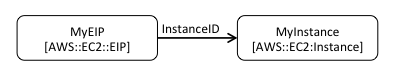
\includegraphics[height=2cm,natwidth=396,natheight=78]{./exaws.png}
\caption{A Simple Example Cloud System on AWS}
\label{fig:exampleaws}
\end{figure}
Note that an Elastic Compute Cloud instance (EC2 instance) is a
virtual machine on AWS IaaS platform and an Elastic IP (EIP)
provides a static IP address for an EC2 instance which is dynamically
created and activated.

%% ===============================================================
\section{OpenStack Heat}
\label{sec:heat}
%% ===============================================================

%% ===============================================================
\section{Puppet, Chef, Ansible}
\label{sec:PCA}
%% ===============================================================

%% ===============================================================
\section{OASIS TOSCA}
\label{sec:TOSCA}
%% ===============================================================
TOSCA is a language to define a {\it service template} for a cloud
system\footnote{TOSCA says a ``service'' to mean a cloud system.}. A
service template consists of a {\it topology template} and optionally
a set of {\it plans}. A topology template defines the resource
structure of a cloud application. Note that a topology template can be
parameterized to give actual environment parameters such as IP
addresses. It is the reason why named as ``template'' and in this
paper we simply say a topology for the sake of brevity. A plan is an
imperative definition of a system operation of the cloud application,
such as a setup plan, written by a standard process modeling language,
such as BPMN.

In TOSCA, a resource is called a {\it node} that has several {\it
  capabilities} and {\it requirements}. A topology consists of a set
of nodes and a set of {\it relationships} of nodes.  A capability is a
function that the node provides to another node, while a requirement
is a function that the node needs to be provided by another node. A
relationship relates a requirement of a source node to a capability of
a target node. Note that nodes and relationships in a topology
template can also be parameterized, thus the exact terms of TOSCA are
node templates and relationship templates.
\begin{figure}
\centering
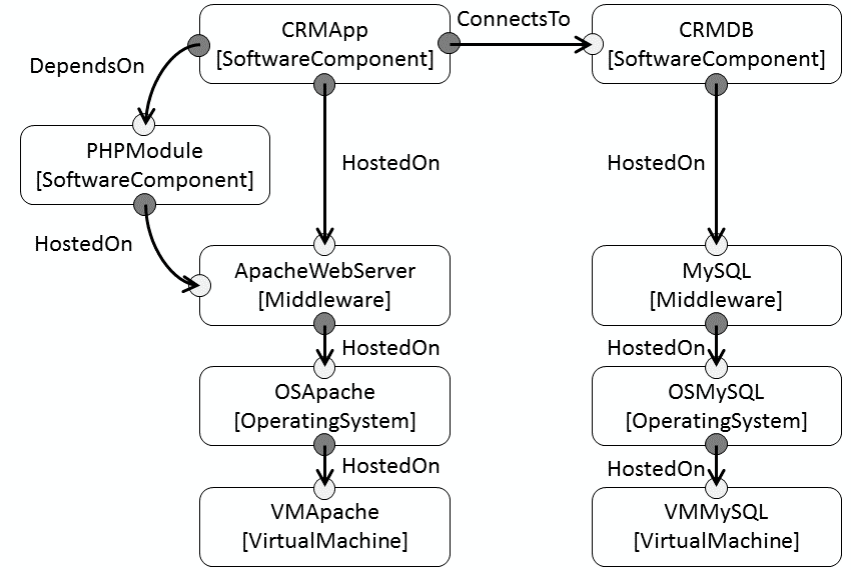
\includegraphics[height=10cm,natwidth=640,natheight=429]{./extopology.png}
\caption{An Example of TOSCA topology}
\label{fig:exampletopology}
\end{figure}
Fig.~\ref{fig:exampletopology} shows a typical example of topology
that consists of nine nodes and nine relationships. White circles
represent capabilities and black ones are requirements.

The current version of TOSCA is an XML-based language. Fig~\ref{fig:topology}
is a part of the topology template of Fig.~\ref{fig:exampletopology}.
\begin{figure}
\centering
\begin{verbatim}
<TopologyTemplate>
  <NodeTemplate id="VMApache" name="VM for Apache" 
                type="VirtualMachine">
    <Capabilities>
      <Capability id="VMApacheOS" name="OS" 
                  type="OperatingSystemContainerCapability"/>
    </Capabilities> </NodeTemplate>
  <NodeTemplate id="OSApache" name="OS for Apache" 
                type="OperatingSystem">
    <Requirements>
      <Requirement id="OSApacheContainer" name="Container" 
                   type="OperatingSystemContainerRequirement"/>
    </Requirements>
    <Capabilities>
      <Capability id="OsApacheSoftware" name="Software" 
                  type="SoftwareContainerCapability"/>
    </Capabilities> </NodeTemplate>
  <RelationshipTemplate id="OSApacheHostedOnVMApache"
                        name="hosted on" type="HostedOn">
    <SourceElement ref="OSApacheContainer"/>
    <TargetElement ref="VMApacheOS"/>
  </RelationshipTemplate>
...
</TopologyTemplate>
\end{verbatim}
\caption{A Topology Template of TOSCA}
\label{fig:topology}
\end{figure}
In this
example, there are two nodes ({\tt VMApache} and {\tt OSApache}) and
one relationship.  A capability is a function that the node provides
to another node, while a requirement is a function that the node needs
to be provided by another node. In this example, {\tt VMApacheOS} is a
capability of {\tt VMApache} and {\tt OSApacheContainer} is a
requirement of {\tt OSApache}.  A relationship relates a requirement
of a source node to a capability of a target node.  Each node,
relationship, capability, and requirement has a type, such as
{\tt VirtualMachine}, {\tt HostedOn}, and so on. Types are main
functionalities of TOSCA that enable reusability of topology
descriptions.

In a typical scenario, a type architect defines and provides several
types of those elements and an application architect uses them to
define a topology of a cloud application. The type architect also
defines operations of node types, such as creating, starting,
stopping, or deleting nodes, and of relationship types, such as
attaching relationships. A system operation of a cloud application is
implemented as an invocation sequence of the type operations, which
can be decided in two kinds of manners. One is an imperative manner in
which the application architect uses a process modeling language to
define a plan that explicitly invokes these type operations. Another is
a declarative one in which the application architect only defines a
topology and a TOSCA tool will automatically invoke appropriate type
operations based on the defined topology. Naturally, the declarative
manner is a main target of OASIS TOSCA because it promotes more
abstract and reusable descriptions of topologies.

In this paper, {\it behavior of topologies} means when
and which type operations should be invoked in automation. It is
important to notice that behavior of a topology depends
on types of included nodes and relationships. We also say
{\it behavior of a type} to mean that the conditions and
results of invoking its type operations, which is defined by a type
architect. Usually, different types of nodes are provided by different
vendors and so specified by different type architects. An application
architect is responsible for behavior of a topology
whereas type architects are responsible for behavior of
their defined types.

Currently there are no practical implementations of the declarative
manner of TOSCA and one of the reasons is that no standard set of type
operations of nodes or relationships are defined and there is no way
for type architects to define behavior of their own types.

%% ===============================================================
\chapter{Preliminaries of \cafeobj}
\label{chap:pre}
%% ===============================================================
\cafeobj\cite{cafeobj} is a formal specification language that is one
of the state-of-the-art algebraic specification languages and a member
of the {\sf OBJ}~\cite{OBJ} language family, such as {\sf
  Maude}~\cite{Maude14}.  \cafeobj specifications are executable by
regarding equations and transition rules in them as left-to-right
rewrite rules, and this executability can be used for interactive
theorem proving.

%% ===============================================================
\section{Modules and Equations}
\label{sec:module}
%% ===============================================================
Basic units of specifications in \cafeobj are {\it modules}.  A
module\footnote{\cafeobj modules can be classified into tight modules
  and loose modules. Roughly speaking, a tight module denotes a unique
  model, while a loose module denotes a class of modules. Those are
  declared with {\tt module!} and {\tt module*} respectively.}
consists of declarations of {\it module importations, sorts, sub-sort
  relations, operators, variables, equations} and {\it transition
  rules}, some of which may be omitted. Conventionally, names of
modules, sorts, and variables are capitalized while names of operators
including constants start with lower case letters or use punctuation
symbols.

Modules may have {\it parameters} and are called parameterized modules
if so. An example of parameterized modules is as follows
\footnote{In \cafeobj, a comment starts with {\tt --} or {\tt **} to
  the end of the line.}:
\begin{verbatim}
module! SET(X :: TRIV) {
  -- Module Importation
  protecting(NAT)

  -- Sorts, Sub-sort Relations
  [Elt.X < Set]

  -- Operators
  op empty : -> Set {constr}
  op _ _ : Set Set -> Set {constr assoc comm idem id: empty}

  op #_ : Set -> Nat
  op _U_ : Set Set -> Set
  op _\in_ : Elt.X Set -> Bool
  op _A_ : Set Set -> Set
  op _\\_ : Set Set -> Set
  op subset : Set Set -> Bool

  -- Variables
  vars S S1 S2 : Set
  vars E E1 : Elt.X

  -- Equations
  -- for =
  eq ((E S1) = (E S2)) = (S1 = S2) .
  -- for empty
  eq ((E S) = empty) = false .
  -- for #_
  eq # empty = 0 .   
  eq # (E S) = 1 + (# S) . 
  -- for _U_
  eq S1 U S2 = S1 S2 .
  -- for _\in_
  eq E \in empty = false .
  eq E \in (E S) = true .
  ceq E \in (E1 S) = E \in S if not(E = E1) .
  -- for _A_
  eq empty A S2 = empty .
  eq (E S1) A (E S2) = E (S1 A S2) .
  ceq (E S1) A S2 = S1 A S2 if not(E \in S2) .
  -- for _\\_ 
  eq empty \\ E = empty .
  eq (E S) \\ E = S .
  ceq (E1 S) \\ E = (E1 (S \\ E)) if not (E = E1) .
  -- for subset
  eq subset(empty,S) = true .
  eq subset((E S1),S2) = E \in S2 and subset(S1,S2) .
}
\end{verbatim}
This module specifies generic sets and has one parameter {\tt X}
constrained by the built-in module {\tt TRIV} in which one sort
{\tt Elt} is only declared as follows:
\begin{verbatim}
module* TRIV {
  [Elt]
}
\end{verbatim}
The sort is referred by {\tt Elt.X} and used for elements in
{\tt SET}. The built-in module {\tt NAT} in which natural numbers are
specified is imported with {\tt protecting}. Modules also can be
imported with {\tt extending} and {\tt using}. {\tt protecting} means
that it is not allowed to add and collapse elements of the imported
modules.  {\tt extending} means it is allowed only to add but not to
collapse them. {\tt using} means it is allowed to add and collapse
them.

One sort {\tt Set} is declared and it is also declared that
{\tt Elt.X} is a sub-sort of {\tt Set}. This is why an element is also
a singleton set that only consists of the element. Operators may be
constructors and a constructor without arguments is a constant. The
operator {\tt empty} is a constant of {\tt Set} and the juxtaposition
operator {\tt \_ \_} is a constructor of {\tt Set}, where an
underscore is the place where an argument is put. It is also specified
that the juxtaposition operator is associative, commutative, and
idempotent and has {\tt empty} as its identity. Operators are defined
with equations. The first equation specifies that \stt{\# empty} equals
{\tt 0}, and the second one specifies that \stt{\# (E S)} equals \stt{1
  + (\# S)}. Those two equations define operator {\tt \#\_} that
counts the number of the elements in a given set. Operators
{\tt \_U\_}, {\tt \_$\backslash$in\_}, {\tt \_A\_}, and {\tt \_$\backslash$\_} are
defined which mean union($\cup$), inclusion($\in$),
intersection($\cap$), and difference($\backslash$) of sets respectively.

Parameterized modules can be instantiated with modules as actual
parameters through\\ views. Let us consider the following module
as an actual parameter of {\tt Set}:
\begin{verbatim}
module! SERVICE {
 protecting(NAT)
 [LocalState Service]
 ops closed open ready : -> LocalState {constr}
 op sv : Nat LocalState -> Service {constr}
}
\end{verbatim}
in which two sorts are declared.  A term of sort {\tt LocalState}
represents a local state of a service and there are three constants of
local states; {\tt closed}, {\tt open}, and {\tt ready}.  A term of
sort {\tt Service} represents a service which has a form
\stt{sv(n,lst)} where {\tt n} is some natural number as an identifier
and {\tt lst} is one of local states.  {\tt SET} can be instantiated
as {\tt SV-SET} as follows:
\begin{verbatim}
module! SV-SET {
 protecting(
  SET(SERVICE{sort Elt -> Service})
   * {sort Set -> SvSet,
      op empty -> empSvSet})
}
\end{verbatim}
What follows {\tt SERVICE}, namely \stt{\{sort Elt -> Service\}}, is
the view used here saying that {\tt Elt} is replaced with
{\tt Service} in the instantiation of {\tt SET} with
{\tt SERVICE}. What follows {\tt *} is renaming. {\tt Set} and
{\tt empty} are renamed as {\tt SvSet} and {\tt empSvSet},
respectively. Other operators are used without renaming.
The instantiated {\tt SET} with {\tt SERVICE} in which {\tt Set} and
{\tt empty} are renamed as mentioned is imported with {\tt protecting}
in {\tt SV-SET}. Command {\tt open} make a given module, {\tt SV-SET}
in this case, available.
\begin{verbatim}
open SV-SET .
 reduce #(sv(1,closed) sv(2,open)) . -- to 2.

 op svs : -> SvSet .
 reduce #(sv(1,closed) svs) = # svs + 1 . -- to true.
close
\end{verbatim}
In {\tt SV-SET}, \stt{(sv(1,closed) sv(2,open))} is a term of sort
{\tt SvSet} and represents a set of services consists of two elements.
Thus, \stt{\#(sv(1,closed) sv(2,open))} is a term of {\tt Nat} which
reduces to {\tt 2} using equations of {\tt SET} as left-to-right
rewrite rules. When {\tt svs} is a term of sort {\tt SvSet},
\stt{(sv(1,closed) svs)} is also a term of sort {\tt SvSet} which
represents a set of services including at least one {\tt closed}
service where {\tt svs} represents the rest of the set. Thus,
\stt{\#(sv(1,closed) svs)} reduces to \stt{\# svs + 1}.

%% ===============================================================
\section{Transition Rules}
\label{sec:rules}
%% ===============================================================
Let us consider the following module:
\begin{verbatim}
module! UPDATE {
 using(SV-SET)

 [State]
 op < _ > : SvSet -> State {constr}
 var SVS : SvSet    
 var N : Nat

 trans [c2o]: 
  < sv(N,closed) SVS > => < sv(N,open) SVS > .

 ctrans [o2r]: 
  < sv(N,open) SVS > => < sv(N,ready) SVS >
  if # SVS > 0 . 
}
\end{verbatim}
Module {\tt UPDATE} specifies a state machine. We say a ``global state''
as a state of the state machine in order to avoid the confusion with
local states of services. A ground term of sort {\tt State} represents
a global state consisting of a set of services, where the set
\{$\ \mbstt{<}\ svs\ \mbstt{>}\mid svs$ is a ground term of {\tt
  SvSet}\} represents the state space. Two transition rules, labeled
by {\tt c2o} and {\tt o2r}, define the state transition over the
states.  Transition rule {\tt c2o} specifies that a {\tt closed}
service appearing in a state is changed to {\tt open}, and {\tt o2r}
specifies that an {\tt open} service is changed to {\tt ready} if
there is at least one other service; {\tt ctrans} means ``conditional
trans''.  Command {\tt execute} makes \cafeobj try to apply transition
rules until no one can be applied.
\begin{verbatim}
open UPDATE .
 execute < sv(1,closed) sv(2,open) > .
   -- to < sv(1,ready)  sv(2,ready) > .

 execute < sv(1,closed) > .
   -- to < sv(1,open) > .
close
\end{verbatim}
Rule {\tt c2o} makes state \stt{<~sv(1,closed)~sv(2,open)~>} transit
to \stt{<~sv(1,open)~sv(2,open)~>} then rule {\tt o2r} makes transit
it to \stt{<~sv(1,ready)~sv(2,open)~>} and successively makes it
transit to \stt{<~sv(1,open)~sv(2,open)~>}. On the other hand,
only rule {\tt c2o} can be applied to state \stt{<~sv(1,closed)~>}
because it has only one element.

%% ===============================================================
\subsection{Formalization of State Machines in \cafeobj}
\label{sec:statemachine}
%% ===============================================================
This section summarizes the formal definitions of state machines in
\cafeobj. Please refer to \cite{Futatsugi15} for detailed
definitions.
\begin{definition}[transition rule]
  Let {\tt State} be a sort of global states, $l$ and $r$ be terms of
  sort {\tt State}, and let $c$ be a term of sort {\tt Bool}, then a
  triple $R = [l,r,c]$ is called a \ul{transition rule} and
  represented as ``\stt{ctrans $l$ => $r$ if $c$ .}''~(or ``\stt{trans
    $l$ => $r$ .}'' when $c$ is \stt{true}).
\end{definition}
\begin{definition}[transition]
  Let $St$ be a set of global states (i.e. ground terms of sort {\tt
    State}), $Rule$ be a set of transition rules, then a pair of
  global states $(S,S')\in Tr\subseteq St\times St$ is called a
  \ul{transition specified by} $Rule$ iff there exists a transition
  rule $R=[l,r,c]\in Rule$ and some ground substitution $\sigma$ such
  that $S=l\sigma$, $S'=r\sigma$, and $c\sigma$ reduces to $true$. We
  also say $R$ \ul{can be applied to} $S$ and say $S'$ is a \ul{next
    state} of $S$.
\end{definition}
\begin{definition}[state machine]
  Let $Rule$ be a set of transition rules, then a \ul{state machine}
  is a triple $(St,Tr,In)$ where $St$ is a set of global state,
  $Tr\subseteq St\times St$ is a set of transitions specified by
  $Rule$, and $In \subseteq St$. An element of $In$ is called an
  \ul{initial state}.
\end{definition}
\begin{definition}[transition sequence]
  Let $(St,Tr,In)$ be a state machine, then a transition sequence is a
  sequence of global states $(S_0,S_1,\dots,S_n)$ where each adjacent
  pair $(S_i,S_{i+1}) \in Tr$. 
\end{definition}
\begin{notation}[$S\alpha,\alpha S,\alpha\beta$]
  Let $S$ be a global state and $\alpha=(S_0,S_1,\dots,S_n)$ be a
  transition sequence, then \ul{$S\alpha$} is the transition sequence
  such that $S\alpha=(S,S_0,S_1,\dots,S_n)$.  \ul{$\alpha S$} is the
  transition sequence such that $\alpha S=(S_0,S_1,\dots,S_n,S)$.  Let
  $\alpha=(S_0,S_1,\dots,S_n)$ and
  $\alpha=(S_{n+1},S_{n+2},\dots,S_{n+m})$ be transition sequences,
  then \ul{$\alpha\beta$} is the transition sequence such that
  $\alpha\beta=(S_0,S_1,\dots,S_n,S_{n+1},S_{n+2},\dots,S_{n+m})$.
\end{notation}
\begin{definition}[reachable]
  Let $(St,Tr,In)$ be a state machine, then a global state $S\in St$
  is \ul{reachable} iff there exists a transition sequence
  $(S_0,S_1,\dots,S_n)$ where $S_0\in In$ and $S=S_n$. Note that $S_0\in
  In$ is reachable because $(S_0)$ is a transition sequence with $n=0$.
\end{definition}
\begin{definition}[invariant]
  Let $(St,Tr,In)$ be a state machine, then a global state predicate
  $p$ is an \ul{invariant} iff $p(S)=true$ holds for any reachable
  state $S$.
\end{definition}

%% ===============================================================
\section{Search Predicates}
\label{sec:searchpredicate}
%% ===============================================================
What is called search predicates can be used to conduct
reachability analysis for such state machines specified in
\cafeobj. Let us consider the following code fragment:
\begin{verbatim}
open UPDATE .
 reduce < sv(1,closed) sv(2,open) > =(*,1)=>+ < SVS > .  -- to true.
 reduce < sv(3,closed) sv(4,ready) > =(*,1)=>+ < SVS > . -- to true.
 reduce < sv(5,open) > =(*,1)=>+ < SVS > .               -- to false.
close
\end{verbatim}
By reducing the term in the code fragment, \cafeobj finds any next
states of the given state, such as
\stt{<~sv(1,open)~sv(2,open)~>}\footnote{{\tt *}, {\tt 1}, and {\tt +}
  specify the range of search. If {\tt 2} is used instead of {\tt *},
  \cafeobj tries to find at most two next states. If {\tt 3} is used
  instead of {\tt 1}, \cafeobj finds all states reachable from the
  given state with at most three state transitions. If {\tt *} is used
  instead of {\tt +}, \cafeobj also includes the given state as a
  search target.  Only \stt{=(*,1)=>+} is used in this paper.}.  The
first reduction returns true because both transition rules are
applicable.  The second one also returns true but only rule {\tt c2o}
is applicable. The third one returns false.

\cafeobj can find next states of a given state such that some
conditions hold in those next states. Let us consider the following
code fragment\footnote{Since the final part of the {\tt reduce} sentence,
  {\tt \{~true~\}}, is for debugging, please ignore it.}:
\begin{verbatim}
open UPDATE .
 pred anyOpen : SvSet .
   -- The same as: op anyOpen : SvSet -> Bool .
 eq anyOpen(sv(N,open) SVS) = true .
 var CC : Bool .
 reduce 
  < sv(1,closed) sv(2,open) > =(*,1)=>+ < SVS > if CC
    suchThat CC implies anyOpen(SVS) { true } .        -- to true.
\end{verbatim}
Here, {\tt pred} declares a predicate, i.e., an operator whose coarity
is {\tt Bool}.  The reduction returns true in which \cafeobj finds any
next states of the given state such that an {\tt open} service is
appearing. In this case, transition rule {\tt c2o} makes such next
state.  Note that when the predicate tries a conditional transition
rule, it binds the rule's condition to {\tt CC}. The {\tt suchThat}
clause uses {\tt CC} to check \stt{anyOpen(SVS)} only when the rule is
applied.

On the other hand, when we want to check some condition holds in all
possible next states, we need some trick. The following code fragment
checks whether all possible next states of state
\stt{<~sv(1,closed)~sv(2,open)~>} include at least one {\tt open} services:
\begin{verbatim}
 reduce not (
  < sv(1,closed) sv(2,open) > =(*,1)=>+ < SVS > if CC
    suchThat not ((CC implies anyOpen(SVS)) == true) { true } ) .
                                                       -- to false.
\end{verbatim}
This style of coding is we call the {\it double negation idiom}
because it returns true when it CANNOT find any next state of the
given state such that NO open service is appearing. The reduction
proceeds as follows:
\begin{enumerate}
\item Try to match LHS of {\tt c2o} to the given state.
\item Also try to match the rule's condition (i.e.\ {\tt true} because
  the rule is unconditional) to {\tt CC} and the substituted RHS
  (i.e.\ \stt{<~sv(1,open)~sv(2,open)~>}) to \stt{<~SVS~>}.
\item Evaluate the substituted {\tt suchThat} clause which reduces to
  false \\ because \stt{anyOpen(sv(1,open) sv(2,open))} reduces to
  true.
\item Then, continuing the search, try to match LHS of {\tt o2r} to
  the given state, the condition (i.e.\ \stt{\# SVS > 0}) to {\tt CC},
  and the substituted RHS (i.e.\ \stt{<~sv(2,ready)~sv(1,closed)~>}) to
  \stt{<~SVS~>}.
\item Evaluate the substituted {\tt suchThat} clause which reduces to
  true because \stt{sv(2,ready) sv(1,closed)} does not include any
  open service.
\item Then the search predicate returns true and the whole term
  reduces to false.
\end{enumerate}
This means that there is a next states of state
\stt{<~sv(1,closed)~sv(2,open)~>} which does not include any {\tt open}
services; \cafeobj finds that it is state
\stt{<~sv(1,closed)~sv(2,ready)~>}.

Note that this is a typical example where we need \stt{\_ == true}. In
\cafeobj, $term1$ {\tt ==} $term2$ reduces to {\tt true} if both terms
are reduced to be the same term and to {\tt false} otherwise. On the
other hand, $term1$ {\tt =} $term2$ reduces to {\tt true} iff $term1$
{\tt ==} $term2$ reduces to {\tt true}. The following code fragment
shows difference between \stt{\_ = \_} and \stt{\_ == \_ }.
\begin{verbatim}
 reduce anyOpen(sv(1,closed)) = true .
                              -- to anyOpen(sv(1,closed)) = true .
 reduce anyOpen(sv(1,closed)) == true . 
                              -- to false.
\end{verbatim}
In this case, \cafeobj cannot decide \stt{anyOpen(SVS)} does or does
not hold because the definition of {\tt anyOpen} is incomplete and
thus the first sentence above can reduce to neither {\tt true} nor
{\tt false}.  The second one using \stt{\_ == true} reduces to
{\tt false}, which is the reason why {\tt suchThat} clause in the
double negation idiom works as we intended.

%% ===============================================================
\subsection{Formalization of Search Predicates}
\label{sec:formalSeach}
%% ===============================================================
This section describes the search predicates more formally.  
\begin{definition}[unconditional search predicate]
  Let $Rule$ be a set of transition rules and let $S$ and $S'$ be
  terms of sort {\tt State}. The \ul{unconditional search predicate,
    $FS(S,S')$} is represented as ``\stt{$S$ =(*,1)=>+ $S'$}''
  and holds iff there exists a transition rule $R=[l,r,c]\in Rule$ and
  a substitution $\sigma$ such that $S\sigma=l\sigma$ holds,
  $S'\sigma=r\sigma$ holds, and $c\sigma$ reduces to true.
\end{definition}
\begin{definition}[conditional search predicate]
  Let $Rule$ be a set of transition rules, $S$ and $S'$ be terms of
  sort {\tt State}, and $CC$ and $B$ be terms of sort {\tt Bool}. The
  \ul{conditional search predicate}, \ul{$CFS(S,S',CC,B)$} is
  represented as ``\stt{$S$ =(*,1)=>+ $S'$ if $CC$ suchThat $B$ \{
    $debug\_info$ \}}''\\ and holds iff there exists a transition
  rule $R=[l,r,c]\in Rule$ and a substitution $\sigma$ such that
  $S\sigma=l\sigma$ holds, $S'\sigma=r\sigma$ holds,
  $CC\sigma=c\sigma$ holds, and $B\sigma$ reduces to true.
\end{definition}

%% ===============================================================
\section{Verification by Proof Scores}
\label{sec:pscore}
%% ===============================================================
A {\it proof score} is an executable specification in \cafeobj such
that if executed as expected, then the desired theorem is
proved~\cite{FutatsugiGO12pps}. Verification by proof scores is an
interactive developing process to think through meaning of the
specification that is very important aspect of developing trusted
systems.

For example, let us verify that in module {\tt UPDATE} there should be
a next state of state $S$ when at least two services included in $S$
are not {\tt ready}.
\begin{verbatim}
module! ProofUPDATE {
 protecting(UPDATE)

 -- Theorem to be proved.
 pred theorem : State

 vars N N1 N2 : Nat
 vars St1 St2 : LocalState .
 vars SVS SVS' : SvSet

 eq theorem(< sv(N1,St1) sv(N2,St2) SVS >)
   = ((St1 == ready) = false and (St2 == ready) = false)
     implies < sv(N1,St1) sv(N2,St2) SVS > =(*,1)=>+ < SVS' > .

 -- Axiom of Nat
 eq (1 + N > 0) = true .

 -- Arbitrary constants.
 op s : -> State
 ops sv1 sv2 : -> Service
 ops st1 st2 : -> LocalState
 ops n1 n2 : -> Nat
 op svs : -> SvSet
}
\end{verbatim}
Module {\tt ProofUPDATE} gets ready for verification; it defines the
theorem to be proved and declares several arbitrary constants.  Note
that we requires an axiom for natural numbers which says that the
successor of a natural number is greater than 0.

Firstly, we begin with the most general case; the state is
\stt{<~sv1~sv2~svs~>} where {\tt sv1} and {\tt sv2} are arbitrary
constants of sort {\tt Service} and {\tt svs} is of {\tt SvSet}.
\begin{verbatim}
-- The most general case.
open ProofUPDATE .
 eq s = < sv1 sv2 svs > .
 reduce theorem(s) . -- to false.
close
\end{verbatim}
This case is too general to judge whether the theorem does or does not
hold.  We should split the case into cases which collectively cover
the general case.  There are three case; (1) both services are closed,
(2) both services are open, and (3) one service is closed and another
is open. The following is a proof score for the three cases.
\begin{verbatim}
-- Case 1: Both services are closed.  
open ProofUPDATE .
 eq s = < sv1 sv2 svs > .  
 eq sv1 = sv(n1,closed) .  
 eq sv2 = sv(n2,closed) .
 reduce theorem(s) . -- to true.  
close

-- Case 2: Both services are open.
open ProofUPDATE .
 eq s = < sv1 sv2 svs > .
 eq sv1 = sv(n1,open) .
 eq sv2 = sv(n2,open) .
 reduce theorem(s) . -- to true.
close

-- Case 3: A closed service and an open service.
open ProofUPDATE .
 eq s = < sv1 sv2 svs > .
 eq sv1 = sv(n1,closed) .
 eq sv2 = sv(n2,open) .
 reduce theorem(s) . -- to true.
close
\end{verbatim}
Verification is successfully done because all cases collectively covering
the most general case are proved.
%% ===============================================================
\section{Constructor-based Inductive Theorem Prover (CITP)}
\label{sec:CITP}
%% ===============================================================
As described above, interactive theorem proving is a systematic
process to split general cases into collectively covering cases until
all cases are specific enough to be proved. Thus, a proof score should
be written more carefully when case splitting becomes deeper. It
sometimes causes to carelessly forget some cases to be proved. In
fact, it may take considerable time to convince that the three cases in
the previous section collectively cover all cases.

In order to assist to develop proof scores which are more systematic
and easier to understand, \cafeobj provides CITP method consisting of
several special commands. The following is a list of part of CITP
commands\footnote{As its name suggests, CITP has capability to
  automatically produce inductive goals based on constructors, however
  we use it only for management of proof trees in this paper.}:
\begin{itemize}
\item \stt{:goal \{eq $term$ = true .\}}\\ Define the goal to be
  proved and let it be the current case. Multiple goal equations
  can be specified.
\item \stt{:ctf \{eq $LHS$ = $RHS$ .\}}\\
  Split the current case into two case adding \stt{eq~$LHS$~=~$RHS$~.} to one case and\\
  \stt{eq~($LHS$~=~$RHS$)~=~false~.} to another.
\item \stt{:csp \{eq $LHS_1$ = $RHS_1$ . eq $LHS_2$ = $RHS_2$ . $\dots$\}}\\
  Split the current case into cases each of which
  \stt{eq~$LHS_i$~=~$RHS_i$~.~} is added to.
\item \stt{:apply (rd)}\\
 Reduce the goal in the current case.
\item \stt{:def $name$ = :ctf \{$\dots$\}}\\
  \stt{:def $name$ = :csp \{$\dots$\}}\\
  Name the case splitting.
\item \stt{:apply ($name_1\ name_2$)}\\ Combine named case
  splittings. When $name_1$ splits $n$ cases and $name_2$ splits $m$
  case, the current case is split into totally $n\times m$ cases.  It
  can also specify {\tt rd}, i.e.\ \stt{:apply~($n_1\ n_2$~rd)}, which
    means to reduce the goal in every split case.
\item \stt{:init [$label$] by \{ $substitution$ \}}\\
  Introduce a $labeled$ lemma proven by other proof scores. $Substitution$ specifies
  how to unify the lemma to the current case. Detailed examples will be explained
  in Chapter~\ref{chap:verification}.
\item \stt{describe proof}\\
 Describe the proof tree consisting of split cases. Proven cases are shown by ``*'' marks.
\item \stt{show proof}\\
Summarize the proof tree consisting of split cases. Proven cases are shown by ``*'' marks.
\end{itemize}

The following is a proof score of CITP version of the example in the previous section:
\begin{verbatim}
select ProofUPDATE .
:goal {
  eq theorem(< sv(n1,st1) sv(n2,st2) svs >) = true .
}
:def csp-st1 = :csp {
 eq st1 = closed .
 eq st1 = open .
 eq st1 = ready .
}
:def csp-st2 = :csp {
 eq st2 = closed .
 eq st2 = open .
 eq st2 = ready .
}
:apply (csp-st1 csp-st2 rd)
describe proof
\end{verbatim}
Command {\tt select} is similar to {\tt open} except that it does not
allow to declare new sorts, operators, equations, and so on. 

Firstly, the goal to be proved should represent the most general case.
Note that predicate {\tt theorem} is defined by only one equation,
which implicitly means that it does not hold for global states which
does not match the LHS of the rule,
i.e.\ \stt{<~sv(N1,St1)~sv(N2,St2)~SVS~>}. Thus, the state in the most
general case is \stt{<~sv(n1,st1)~sv(n2,st2)~svs~>} where \stt{n1,
  st1, n2, st2}, and {\tt svs} are arbitrary constants of
corresponding classes.  Then, since class {\tt LocalState} has only
three constants ({\tt closed, open} , and {\tt ready}) as constructors
in module {\tt UPDATE}, there are three cases where {\tt st1} (and
also {\tt st2}) is one of the three constants in each of cases. Thus
the combination of case splitting for {\tt st1} and {\tt st2}
collectively covers all cases.

The final command, \stt{describe proof}, describes the proof tree as
follows:
\begin{verbatim}
==> root*
    -- context module: #Goal-root
    -- targeted sentence:
      eq theorem(< (sv(n1, st1) sv(n2, st2) svs) >)
          = true .
[csp-st1] 1*
    -- context module: #Goal-1
    -- assumption
      eq [csp-st1]: st1 = closed .
    -- targeted sentence:
      eq theorem(< (sv(n1, st1) sv(n2, st2) svs) >)
          = true .
[csp-st2] 1-1*
    -- context module: #Goal-1-1
    -- assumptions
      eq [csp-st1]: st1 = closed .
      eq [csp-st2]: st2 = closed .
    -- discharged sentence:
      eq [RD]: theorem(< (sv(n1, st1) sv(n2, st2) svs) >)
          = true .
[csp-st2] 1-2*
    -- context module: #Goal-1-2
    -- assumptions
      eq [csp-st1]: st1 = closed .
      eq [csp-st2]: st2 = open .
    -- discharged sentence:
      eq [RD]: theorem(< (sv(n1, st1) sv(n2, st2) svs) >)
          = true .
[csp-st2] 1-3*
    -- context module: #Goal-1-3
    -- assumptions
      eq [csp-st1]: st1 = closed .
      eq [csp-st2]: st2 = ready .
    -- discharged sentence:
      eq [RD]: theorem(< (sv(n1, st1) sv(n2, st2) svs) >)
          = true .
[csp-st1] 2*
    -- context module: #Goal-2
    -- assumption
      eq [csp-st1]: st1 = open .
    -- targeted sentence:
      eq theorem(< (sv(n1, st1) sv(n2, st2) svs) >)
          = true .
[csp-st2] 2-1*
    -- context module: #Goal-2-1
    -- assumptions
      eq [csp-st1]: st1 = open .
      eq [csp-st2]: st2 = closed .
    -- discharged sentence:
      eq [RD]: theorem(< (sv(n1, st1) sv(n2, st2) svs) >)
          = true .
[csp-st2] 2-2*
    -- context module: #Goal-2-2
    -- assumptions
      eq [csp-st1]: st1 = open .
      eq [csp-st2]: st2 = open .
    -- discharged sentence:
      eq [RD]: theorem(< (sv(n1, st1) sv(n2, st2) svs) >)
          = true .
[csp-st2] 2-3*
    -- context module: #Goal-2-3
    -- assumptions
      eq [csp-st1]: st1 = open .
      eq [csp-st2]: st2 = ready .
    -- discharged sentence:
      eq [RD]: theorem(< (sv(n1, st1) sv(n2, st2) svs) >)
          = true .
[csp-st1] 3*
    -- context module: #Goal-3
    -- assumption
      eq [csp-st1]: st1 = ready .
    -- targeted sentence:
      eq theorem(< (sv(n1, st1) sv(n2, st2) svs) >)
          = true .
[csp-st2] 3-1*
    -- context module: #Goal-3-1
    -- assumptions
      eq [csp-st1]: st1 = ready .
      eq [csp-st2]: st2 = closed .
    -- discharged sentence:
      eq [RD]: theorem(< (sv(n1, st1) sv(n2, st2) svs) >)
          = true .
[csp-st2] 3-2*
    -- context module: #Goal-3-2
    -- assumptions
      eq [csp-st1]: st1 = ready .
      eq [csp-st2]: st2 = open .
    -- discharged sentence:
      eq [RD]: theorem(< (sv(n1, st1) sv(n2, st2) svs) >)
          = true .
[csp-st2] 3-3*
    -- context module: #Goal-3-3
    -- assumptions
      eq [csp-st1]: st1 = ready .
      eq [csp-st2]: st2 = ready .
    -- discharged sentence:
      eq [RD]: theorem(< (sv(n1, st1) sv(n2, st2) svs) >)
          = true .
\end{verbatim}
This means that the most general case ({\tt root}) is split into three
cases ({\tt 1}, {\tt 2}, and {\tt 3}) using {\tt csp-st1} each of
which is also split into three case (for example, {\tt 1-1},
{\tt 1-2}, and {\tt 1-3}) using {\tt csp-st2}.  ``*'' marks show the
all cases are successfully proved.

%% ===============================================================
\chapter{Models and Representations of Cloud Orchestration}
\label{chap:model}
%% ===============================================================
Cloud Orchestration is automation of operations such as set-up,
scale-out, scale-in, or shutdown of cloud systems. In order to verify
correctness of an automated operation of a cloud system, we need to
model the structure of the target cloud system and the behavior of the
operation. We say ``model'' which means to abstractly and formally
specify the structure and behavior. A specified model is represented
by a formal specification language, i.e.\ \cafeobj in this paper.

%% ===============================================================
\section{Structure Models and Representations}
\label{sec:structuremodel}
%% ===============================================================
CloudFormation models a structure of a cloud system simply as a set
of {\it resources} on IaaS platform of AWS. The model is called a {\it
  template} which is represented by JSON as illustrated in
Fig.~\ref{fig:AWSExample}.  A resource has an identifier and a type
and includes several {\it properties} which may depend on other
resources.

On the other hand, TOSCA's model of a cloud system is more structured
to manage any types of cloud resources, as well as inside VMs, and any
types of operations such as scale-out, scale-in, shutdown, and so on.
A TOSCA's model, called a {\it topology}, which is represented by XML
as illustrated in Fig~\ref{fig:topology}. A topology consists of a set
of {\it nodes} and a set of {\it relationships} between nodes. A node
has several {\it capabilities} and {\it requirements}. A relationship
relates a requirement of a source node to a capability of a target
node.

In order to cover many different kinds of models of cloud system
structures, our framework provides a generic model of a cloud system
structure which consists of several {\it classes} of {\it
  objects}. For example, in the case of CloudFormation, a cloud system
consists of two classes (resource and property) of objects whereas
TOSCA models that a cloud system consists of four classes (node,
relationship, capability, and requirement). For a while, we explain
our framework using the simple CloudFormation template shown in
Fig.~\ref{fig:AWSExample} and the case of TOSCA topologies will be
explained in Chapter~\ref{chap:appTOSCA}.

An object has a {\it type}\footnote{Do not think a {\it type} is that
  of programming languages which is called {\it sort} in \cafeobj. A
  type is just an attribute of an object. We use the term because both
  CloudFormation and TOSCA use it.}, an {\it identifier}(ID), a {\it
  local state}, and possibly {\it links} to other objects. In the case
of the example show in Fig.~\ref{fig:AWSExample}, a resource object
whose type is AWS::EC2::Instance has its ID as MyInstance. The type of
MyEIP resource is AWS::EC2::EIP. MyEIP has a property but its ID is
hidden and we assume it is MyEIP::InsID since its parent is MyEIP and
its type is InstanceId. MyEIP::InsID has a link to MyInstance. Local
states of objects are used for automation of operations, which will be
explained in Section~\ref{sec:behaviormodel}. Note that a link is
represented by an identifier of the linked object in our framework.

An object belongs to a class and thus a class is a set of objects. We
assume this set consists of countably infinite objects each of which
has its fixed ID and type. Local states or links of objects may be
dynamically changed.  A class decides the set of possible types, the set
of possible local states of its objects. A class also decides how its
objects link to other objects.

Users of the framework should design representation of the system
model in \cafeobj language.  A class is represented as a \cafeobj
module that defines a sort of its objects, a constructor of the sort,
a set of literals of types, and a set of literals of local states.  An
object is represented as a ground constructor term of the sort.

For the example show in Fig.~\ref{fig:AWSExample}, three objects may
be represented as the following ground terms:
\begin{verbatim}
  res(ec2Instance, myInstance, initial)
  res(ec2Eip, myEIP, initial)
  prop(instanceId,myEIP::InsID,notready,myEIP,myInstance)
\end{verbatim}
Although the users of the framework can freely design the
representation of objects, typically the constructor name represents
the class of the object ({\tt res}, {\tt prop}), the first argument is
its type ({\tt ec2Instance}, {\tt ec2Eip}, {\tt instanceId}), the
second is its identifier ({\tt myInstance}, {\tt myEIP},
{\tt myEIP::InsID})\footnote{In this paper, we often use an identifier
  to designate an object which has the identifier for the sake of
  brevity.}, and the third is its local state. In this example, the
initial states of resource and property objects are assumed as
{\tt initial} and {\tt notready} respectively. The fourth argument of the
property object represents a link to its parent, {\tt myEIP}, and the
fifth represents that the property depends on {\tt myInstance}. The
example of \cafeobj modules representing resource and property classes
will be shown in Chapter~\ref{chap:reusable}.

%% ===============================================================
\section{Behavior Models and Representations}
\label{sec:behaviormodel}
%% ===============================================================
The framework models the behavior of an automated operation of a cloud
system as a state machine in which a set of {\it transition rules} of
states specifies the behavior. We say a {\it global state} as a state
of the state machine in order to avoid the confusion with local states
of objects. A global state is a finite set of objects each of which is
included of some class. A transition rule makes a global state transit
to another global state where local states or links of some objects
are changed.

In the case of a template of CloudFormation, a global state consists
of finite number of resources and their properties.  The behavior is
very simple; CloudFormation tries to start all resources according to
the dependency specified by the template.  This can be modeled such
that a local state of a resource is firstly {\it initial} and finally
{\it started} but a dependent resource can be {\it started} after all
resources it depends become {\it started}.  The dependency is
specified such that a property linking some resource is firstly {\it
  notready} and becomes {\it ready} when the linked resource is {\it
  started} and a resource can be {\it started} when all of its
properties become {\it ready}.

A global state is represented in \cafeobj as a ground constructor term
of sort {\tt State}, which is typically a tuple of sets of objects,
each of the sets is a finite subset of a class.  In the case of
CloudFormation, sort {\tt State} is defined as a pair of a set of
resources and a set of properties and the global state shown in
Fig.~\ref{fig:AWSExample} is represented as follows:\footnote{Module
  {\tt LINKS} and several sorts of constants will be explained in the
  next chapter.}
\begin{verbatim}
module! STATE {
  protecting(LINKS)
  [State]
  op <_,_> : SetOfResource SetOfProperty -> State {constr}
}

open STATE . 
 -- Constants
 ops ec2Instance ec2Eip : -> RSTypeLt .
 ops myInstance myEIP : -> RSIDLt .
 ops myEIP::InsID : -> PRIDLt .
 op instanceId : -> PRTypeLt .
 op s0 : -> State .
 eq s0 =
  < (res(ec2Instance, myInstance, initial) res(ec2Eip, myEIP, initial)),
    (prop(instanceId, myEIP::InsID, notready, myEIP, myInstance)) >
\end{verbatim}
The behavior is modeled and represented by a set of two transition
rules as follows:
\begin{verbatim}
module! STATERules {
 protecting(STATEfuns)

 -- Variables
 vars IDRS IDRRS : RSID 
 var IDPR : PRID
 var TRS : RSType
 var TPR : PRType
 var SetRS : SetOfResource
 var SetPR : SetOfProperty

 -- Start an initial resource
 --  if all of its properties are ready.
 ctrans [R01]:
    < (res(TRS,IDRS,initial) SetRS), SetPR >
 => < (res(TRS,IDRS,started) SetRS), SetPR > 
    if allPROfRSInStates(SetPR,IDRS,ready) .

 -- Let a not-ready property be ready 
 --  if its referring resource is started.
 trans [R02]:
    < (res(TRS,IDRRS,started) SetRS), 
      (prop(TPR,IDPR,notready,IDRS,IDRRS) SetPR) >
 => < (res(TRS,IDRRS,started) SetRS), 
      (prop(TPR,IDPR,ready   ,IDRS,IDRRS) SetPR) > .
}
\end{verbatim}
Predicate \stt{allPROfRSInStates(SetPR,IDRS,ready)} checks a set of
properties {\tt SetPR} whether every property of resource {\tt IDRS}
is {\tt ready}, which will be explained in Section~\ref{sec:linkpred}.
Thus, rule {\tt R01} means that an {\tt initial} resource becomes {\tt
  started} when all of its properties are {\tt ready}.  The LHS of
rule {\tt R02} includes a resource and a property.  The second link of
the property is the identifier of the resource, which means the
property refers the resource.  Thus, rule {\tt R02} means that a {\tt
  notready} property becomes {\tt ready} when it refers a {\tt
  started} resource.

%% ===============================================================
\section{Simulation of Models}
\label{sec:simulation}
%% ===============================================================
\cafeobj provides {\tt execute} command to execute a state machine
trying to apply transition rules as long as possible.
\begin{verbatim}
open STATERules .
 -- Constants
 ops ec2Instance ec2Eip : -> RSTypeLt .
 ops myInstance myEIP : -> RSIDLt .
 ops myEIP::InsID : -> PRIDLt .
 op instanceId : -> PRTypeLt .
 op s0 : -> State .
 eq s0 =
   < (res(ec2Instance, myInstance,initial) res(ec2Eip,myEIP,initial)),
     (prop(instanceId,myEIP::InsID,notready,myEIP,myInstance)) > .
      
 execute s0 . 
 -- will be produced 
 -- < (res(ec2Instance, myInstance,started) res(ec2Eip,myEIP,started)),
 --   (prop(instanceId,myEIP::InsID,ready,myEIP,myInstance)) > .
\end{verbatim}
The following is a part of log messages of the execution above, which
shows that firstly rule {\tt R01} makes {\tt myInstance} transit
from {\it initial} to {\it ready}, then {\tt R02} makes
{\tt myEIP::InsID} transit from {\it notready} to {\it ready}, and
finally {\tt R01} makes {\tt myEIP} transit from {\tt initial} to
{\it started}.
\begin{verbatim}
...
1>[2] apply trial #1
-- rule: ctrans [R01]: 
          (< (res(TRS,IDRS,initial) SetRS) , SetPR >) 
       => (< (res(TRS,IDRS,started) SetRS) , SetPR >)
       if allPROfRSInStates(SetPR,IDRS,ready)
    { IDRS |-> myInstance, 
      TRS |-> ec2Instance, 
      SetRS |-> res(ec2Eip,myEIP,initial), 
      SetPR |-> prop(instanceId,myEIP::InsID,notready,myEIP,myInstance)
    }
...
1>[19] match success #1
1<[19] (< (res(ec2Eip,myEIP,initial) res(ec2Instance,myInstance,initial)),
          (prop(instanceId,myEIP::InsID,notready,myEIP,myInstance)) >)
   --> (< (res(ec2Instance,myInstance,started) res(ec2Eip,myEIP,initial)),
          (prop(instanceId,myEIP::InsID,notready,myEIP,myInstance)) >)
1>[20] rule: trans [R02]:
          (< (res(TRS,IDRRS,started) SetRS),
             (prop(TPR,IDPR,notready,IDRS,IDRRS) SetPR) >)
       => (< (res(TRS,IDRRS,started) SetRS),
             (prop(TPR,IDPR,ready,IDRS,IDRRS) SetPR) >)
    { IDPR |-> myEIP::InsID,
      TPR |-> instanceId,
      IDRS |-> myEIP,
      SetPR |-> empPR,
      IDRRS |-> myInstance,
      TRS |-> ec2Instance,
      SetRS |-> res(ec2Eip,myEIP,initial)
    }
1<[20] (< (res(ec2Eip,myEIP,initial) res(ec2Instance,myInstance,started)),
          (prop(instanceId,myEIP::InsID,notready,myEIP,myInstance)) >)
   --> (< (res(ec2Instance,myInstance,started) res(ec2Eip,myEIP,initial)),
          (prop(instanceId,myEIP::InsID,ready,myEIP,myInstance)) >)
1>[21] apply trial #1
...
1>[42] match success #1
1<[42] (< (res(ec2Eip,myEIP,initial) res(ec2Instance,myInstance,started)),
          (prop(instanceId,myEIP::InsID,ready,myEIP,myInstance)) >)
   --> (< (res(ec2Eip,myEIP,started) res(ec2Instance,myInstance,started)),
          (prop(instanceId,myEIP::InsID,ready,myEIP,myInstance)) >)

(< (res(ec2Instance,myInstance,started) res(ec2Eip,myEIP,started)),
   (prop(instanceId,myEIP::InsID,ready,myEIP,myInstance)) >):State
\end{verbatim}

%% ===============================================================
\chapter{General Templates and Predicate Libraries}
\label{chap:reusable}
%% ===============================================================
The framework uses the template mechanism of \cafeobj to provide a
general way to model cloud orchestration, predefined predicate
libraries, and proved lemmas together with their proof scores.
%% ===============================================================
\section{Template Modules of Objects}
\label{sec:objectbase}
%% ===============================================================
Template module {\tt OBJECTBASE} defines nine sorts and more than ten
operators/predicates of objects, which generally and minimally defines
what an object is in a class. The template can be instantiated and
imported in a module for each class of objects, where the imported
sorts and operators can be used only by renaming appropriately. For
the example show in Fig.~\ref{fig:AWSExample}, following module
{\tt RESOURCE} describes specifications of the resource class for
CloudFormation\footnote{{\tt OBJECTBASE} is a template with no
  parameter and is used to instantiate a new module and rename
  predefined sorts/operators.}.
%% =======================================================================
\begin{verbatim}
module! RESOURCE {
  -- Instantiation of Template
  extending(OBJECTBASE
    * {sort Object -> Resource,
       sort ObjIDLt -> RSIDLt,
       sort ObjID -> RSID,
       sort ObjTypeLt -> RSTypeLt,
       sort ObjType -> RSType,
       sort ObjStateLt -> RSStateLt,
       sort ObjState -> RSState,
       sort SetOfObject -> SetOfResource,
       sort SetOfObjState -> SetOfRSState,
       op empObj -> empRS,
       op empState -> empSRS,
       op existObj -> existRS,
       op existObjInStates -> existRSInStates,
       op uniqObj -> uniqRS,
       op #ObjInStates -> #ResourceInStates,
       op getObject -> getResource,
       op allObjInStates -> allRSInStates,
       op allObjNotInStates -> allRSNotInStates,
       op someObjInStates -> someRSInStates}
  )

  -- Constructor
  -- res(RSType, RSID, RSState) is a Resource.
  op res : RSType RSID RSState -> Resource {constr}

  -- Variables
  var TRS : RSType
  var IDRS : RSID
  var SRS : RSState

  -- Selectors
  eq type(res(TRS,IDRS,SRS)) = TRS .
  eq id(res(TRS,IDRS,SRS)) = IDRS .
  eq state(res(TRS,IDRS,SRS)) = SRS .

  -- Local States
  ops initial started : -> RSStateLt {constr}
}
\end{verbatim}
%% =======================================================================
The following is a list of part of sorts and operators predefined by
template module {\tt OBJECTBASE} whereas argument $obj$ is an object,
$id$ is an identifier of an object, $seto$ is a set of objects, and
$setls$ is a set of local states of objects:
\begin{itemize}
\item sort \stt{Object} (as \stt{Resource})\\
  Sort for objects themselves.
\item sort \stt{ObjIDLt} (renamed as \stt{RSIDLt})\\
  Subsort of {\tt ObjID} for identifier literals. A literal is a
  constant for which {\tt OBJECTBASE} predefines a special equality
  predicate such that $\_ = \_$ is exactly the same as $\_ == \_ $ .
\item sort \stt{ObjID} (as \stt{RSID})\\
  Sort for identifiers of objects.
\item sort \stt{ObjTypeLt} (as \stt{RSTypeLt})\\
  Subsort of {\tt ObjType} for type literals.
\item sort \stt{ObjType} (as \stt{RSType})\\
  Sort for types of objects.
\item sort \stt{ObjStateLt} (as \stt{RSStateLt})\\
  Subsort of {\tt ObjState} for local state literals.
\item sort \stt{ObjState} (as \stt{RSState})\\
  Sort for local states of objects.
\item sort \stt{SetOfObject} (as \stt{SetOfResource})\\
  Soft for sets of objects.
\item sort \stt{SetOfObjState} (as \stt{SetOfRSState})\\
  Sort for sets of local states of objects.
\item op \stt{empObj} (as \stt{empRS})\\
  Constant representing an empty set of objects.
\item op \stt{empState} (as \stt{empSRS})\\
  Constant representing an empty set of local states of objects.
\item op \stt{existObj} (as \stt{existRS})\\ 
  Predicate used as \stt{existObj($seto$,$id$)} which holds iff an
  object with identifier $id$ is included in $seto$;\\$~~~~\exists o\in
  seto: \mbstt{id}(o)=id$.
\item op \stt{existObjInStates} (as \stt{existRSInStates})\\
  Predicate used as \stt{existObjInStates($seto$,$id$,$setls$)} which
  holds iff an object with identifier $id$ is included in $seto$ and
  its local state is included in $setls$;\\$~~~~\exists o\in seto:
  (\mbstt{id}(o)=id \land \mbstt{state}(o)\in setls)$.
\item op \stt{uniqObj} (as \stt{uniqRS})\\
  Predicate used as \stt{uniqObj($seto$)} which checks whether the
  identifier of each object is unique in $seto$;\\$~~~~\forall o,o'\in
  seto:(o\ne o'\ra\mbstt{id}(o)\ne\mbstt{id}(o'))$.
\item op \stt{\#ObjInStates} (as \stt{\#ResourceInStates})\\ 
  Operator used as \stt{\#ObjInStates($setls$,$seto$)} which returns
  the number of objects in $seto$ whose local states are
  included in $setls$.
\item op \stt{getObject} (as \stt{getResource})\\ 
  Operator used as \stt{getObject($seto$,$id$)} which returns an
  object in $seto$ whose identifier is $id$.
\item op \stt{allObjInStates} (as \stt{allRSInStates})\\
  Predicate used as \stt{allObjInStates($seto$,$setls$)} which holds iff
  the local states of all objects in $seto$ are included
  in $setls$;\\$~~~~\forall o\in seto:\mbstt{state}(o)\in setls$.
\item op \stt{allObjNotInStates} (as \stt{allRSNotInStates})\\
  Predicate used as \stt{allObjNotInStates($seto$,$setls$)} which holds iff
  the local states of all objects in $seto$ are not included
  in $setls$;\\$~~~~\forall o\in seto:\mbstt{state}(o)\not\in setls$.
\item op \stt{someObjInStates} (as \stt{someRSInStates})\\ 
  Predicate used as \stt{someObjInStates($seto$,$setls$)} which holds
  iff there exists an objects in $seto$ whose local state is included
  in $setls$;\\$~~~~\exists o\in seto:\mbstt{state}(o)\in setls$.

\end{itemize}

The module importing the instantiated template can be extended to
freely define a constructor of objects and local state literals.  In
this case, module {\tt RESOURCE} defines a constructor ({\tt res}) of
sort {\tt Resource} whose arguments are a type, an identifier, and a
local state of the resource. It also defines local state literals,
{\tt initial} and {\tt started} of a resource.

In addition, the module should implement three selector operators,
{\tt type}, {\tt id}, and {\tt state}, each of which takes a resource
as an argument and returns the type, the identifier, and the local
state of the resource respectively since {\tt OBJECTBASE} uses them to
implement the predefined general operators\footnote{{\tt OBJECTBASE}
  declares and uses these operators and so {\tt RESOURCE} only should
  define them by equations.}.

Similarly, following module {\tt PROPERTY} specifies the property class 
for the example show in Fig.~\ref{fig:AWSExample}.
%% =======================================================================
\begin{verbatim}
module! PROPERTY {
  protecting(RESOURCE)

  -- Instantiation of Template
  extending(OBJECTBASE
    * {sort Object -> Property,
       sort ObjIDLt -> PRIDLt,
       sort ObjID -> PRID,
       sort ObjTypeLt -> PRTypeLt,
       sort ObjType -> PRType,
       sort ObjStateLt -> PRStateLt,
       sort ObjState -> PRState,
       sort SetOfObject -> SetOfProperty,
       sort SetOfObjState -> SetOfPRState,
       op empObj -> empPR,
       op empState -> empSPR,
       op existObj -> existPR,
       op existObjInStates -> existPRInStates,
       op uniqObj -> uniqPR,
       op #ObjInStates -> #PropertyInStates,
       op getObject -> getProperty,
       op allObjInStates -> allPRInStates,
       op allObjNotInStates -> allPRNotInStates,
       op someObjInStates -> somePRInStates}
  )

  -- Constructor
  -- prop(PRType, PRID, PRState, RSID, RSID) is a Property.
  op prop : PRType PRID PRState RSID RSID -> Property {constr}

  -- Variables
  var TPR : PRType
  var IDPR : PRID
  var SPR : PRState
  vars IDRS1 IDRS2 : RSID

  -- Selectors
  op parent : Property -> RSID
  op refer : Property -> RSID
  eq type(prop(TPR,IDPR,SPR,IDRS1,IDRS2)) = TPR .
  eq id(prop(TPR,IDPR,SPR,IDRS1,IDRS2)) = IDPR .
  eq state(prop(TPR,IDPR,SPR,IDRS1,IDRS2)) = SPR .
  eq parent(prop(TPR,IDPR,SPR,IDRS1,IDRS2)) = IDRS1 .
  eq refer(prop(TPR,IDPR,SPR,IDRS1,IDRS2)) = IDRS2 .

  -- Local States
  ops notready ready : -> PRStateLt {constr}
}
\end{verbatim}
%% =======================================================================
Firstly, module {\tt PROPERTY} imports module {\tt RESOURCE} using
{\tt protecting} because a property object links to its parent
resource and also links to its referring resource.

Module {\tt PROPERTY} defines a constructor ({\tt prop}) of sort
{\tt property} whose arguments are a type, an identifier, a local
state, and links of the property. As noted before, a link is
represented by an identifier of the linked object.  It also defines
local state literals, {\tt notready} and {\tt ready} of a property.

In addition to the mandatory selectors ({\tt type}, {\tt id}, and
{\tt state}), module {\tt PROPERTY} declares and defines two more
selectors, {\tt parent} and {\tt refer}, each of which returns a
parent resource and a referring resource of the property respectively.

%% ===============================================================
\section{Template Modules for Links}
\label{sec:linkpred}
%% ===============================================================
In addition to the operators provided by template module {\tt OBJECTBASE}, two
template modules {\tt OBJLINKMANY2ONE} and {\tt OBJLINKONE2ONE}
provide many predefined operators/predicates for links between
objects. Representing object structures by using links, instead of
nesting structures, enables the framework to be easily applied to any
kinds of model structures and to effectively provide a predefined set
of operators/predicates.

A template module {\tt OBJLINKMANY2ONE} takes one parameter module of
a class whose object links to another object. In order to provide
predefined operators for links, the template module assumes that the
parameter module defines eleven specific sorts and five specific
operators. For example, it assumes that a parameter module defines
{\tt Object} as a sort for linking objects, {\tt LObject} as a sort
for linked objects, {\tt link} as a selector of {\tt Object} which
returns the identifier of linked object, and so on. When the actual
parameter module defines those sorts and operators with the different
names from ones assumed, \cafeobj allows to specify correspondence of
the names. In the case of CloudFormation, the sort for linking objects
is {\tt Property}, the sort for linked objects is {\tt Resource}, and
the selectors are {\tt parent} and {\tt refer} defined by module
{\tt PROPERTY}.  The following module {\tt LINKS} imports
{\tt OBJLINKMANY2ONE} twice for both kinds of links specifying the
correspondence of the names:
%% =======================================================================
\begin{verbatim}
module! LINKS {
  -- A Property links to its parent Resource
  extending(OBJLINKMANY2ONE(
    PROPERTY {sort Object -> Property,
              sort ObjID -> PRID,
              sort ObjType -> PRType,
              sort ObjState -> PRState,
              sort SetOfObject -> SetOfProperty,
              sort SetOfObjState -> SetOfPRState,
              sort LObject -> Resource,
              sort LObjID -> RSID,
              sort LObjState -> RSState,
              sort SetOfLObject -> SetOfResource,
              sort SetOfLObjState -> SetOfRSState,
              op link -> parent,
              op empLObj -> empRS,
              op existLObj -> existRS,
              op existLObjInStates -> existRSInStates,
              op getLObject -> getResource}
    )
    * {op hasLObj -> hasParent,
       op getXOfZ -> getRSOfPR,
       op getZsOfX -> getPRsOfRS,
       op getZsOfXInStates -> getPRsOfRSInStates,
       op getXsOfZs -> getRSsOfPRs,
       op getXsOfZsInStates -> getRSsOfPRsInStates,
       op getZsOfXs -> getPRsOfRSs,
       op getZsOfXsInStates -> getPRsOfRSsInStates,
       op allZHaveX -> allPRHaveRS,
       op allZOfXInStates -> allPROfRSInStates,
       op ifOfXThenInStates -> ifOfRSThenInStates,
       op ifXInStatesThenZInStates -> ifRSInStatesThenPRInStates}
  )

  -- A Property links to its referring Resource
  extending(OBJLINKMANY2ONE(
    PROPERTY {sort Object -> Property,
              sort ObjID -> PRID,
              sort ObjType -> PRType,
              sort ObjState -> PRState,
              sort SetOfObject -> SetOfProperty,
              sort SetOfObjState -> SetOfPRState,
              sort LObject -> Resource,
              sort LObjID -> RSID,
              sort LObjState -> RSState,
              sort SetOfLObject -> SetOfResource,
              sort SetOfLObjState -> SetOfRSState,
              op link -> refer,
              op empLObj -> empRS,
              op existLObj -> existRS,
              op existLObjInStates -> existRSInStates,
              op getLObject -> getResource}
    )
    * {op hasLObj -> hasRefRS,
       op getXOfZ -> getRRSOfPR,
       op getZsOfX -> getPRsOfRRS,
       op getZsOfXInStates -> getPRsOfRRSInStates,
       op getXsOfZs -> getRRSsOfPRs,
       op getXsOfZsInStates -> getRRSsOfPRsInStates,
       op getZsOfXs -> getPRsOfRRSs,
       op getZsOfXsInStates -> getPRsOfRRSsInStates,
       op allZHaveX -> allPRHaveRRS,
       op allZOfXInStates -> allPROfRRSInStates,
       op ifOfXThenInStates -> ifOfRRSThenInStates,
       op ifXInStatesThenZInStates -> ifRRSInStatesThenPRInStates}
    )
}
\end{verbatim}
%% =======================================================================
The following is a list of eleven sorts and five operators assumed by
module {\tt OBJLINKMANY2ONE} whereas argument $obj$ is a linking
object, $lid$ is an identifier of a linked object, $setlo$ is a set of
linked objects, and $setlls$ is a set of local states of linked
objects:
\begin{itemize}
\item sort \stt{Object} (actually named as \stt{Property})\\
  Sort for linking objects.
\item sort \stt{ObjID} (as \stt{PRID})\\
  Sort for identifiers of linking objects.
\item sort \stt{ObjType} (as \stt{PRType})\\
  Sort for types of linking objects.
\item sort \stt{ObjState} (as \stt{PRState})\\
  Sort for local states of linking objects.
\item sort \stt{SetOfObject} (as \stt{SetOfProperty})\\
  Sort for sets of linking objects.
\item sort \stt{SetOfObjState} (as \stt{SetOfPRState})\\
  Sort for sets of local states of linking objects.
\item sort \stt{LObject} (as \stt{Resource})\\
  Sort for linked objects.
\item sort \stt{LObjID} (as \stt{RSID})\\
  Sort for identifiers of linked objects.
\item sort \stt{LObjState} (as \stt{RSState})\\
  Sort for local states of linked objects.
\item sort \stt{SetOfLObject} (as \stt{SetOfResource})\\
  Sort for sets of linked objects.
\item sort \stt{SetOfLObjState} (as \stt{SetOfRSState})\\
  Sort for sets of local states of linked objects.
\item op \stt{link} (as \stt{parent} and \stt{refer})\\
  Selector used as \stt{link($obj$)} which returns the identifier of
  the object linked by $obj$.
\item op \stt{empLObj} (as \stt{empRS})\\
  Constant representing an empty set of linked objects.
\item op \stt{existLObj} (as \stt{existRS})\\
  Predicate used as \stt{existLObj($setlo$,$lid$)} which holds iff an
  linked object with identifier $lid$ is included in
  $setlo$;\\$~~~~\exists lo\in setlo:\mbstt{id}(lo)=lid$.
\item op \stt{existLObjInStates} (as \stt{existRSInStates})\\
  Predicate used as \stt{existLObjInStates($setlo$,$lid$,$setlls$)}
  which holds iff an linked object with identifier $lid$ is included
  in $setlo$ and its local state is included in
  $setlls$;\\$~~~~\exists lo\in setlo:(\mbstt{id}(lo)=lid\land
  \mbstt{state}(lo)\in setlls)$.
\item op \stt{getLObject} (as \stt{getResource})\\
  Operator used as \stt{getLObject($setlo$,$lid$)} which returns an
  object in $setlo$ whose identifier is $lid$.
\end{itemize}
Note that {\tt LINKS} imports {\tt OBJLINKMANY2ONE} twice but only
selector {\tt link} is specified differently, {\tt parent} and {\tt
  refer}, and others are the same.

Many operators/predicates between linking (Z) and linked (X) objects
are provided. In this case, each of them is twice renamed differently.
The following is a list of part of operators predefined by template
module {\tt OBJLINKMANY2ONE} whereas argument $obj$ is a linking
object, $seto$ is a set of linking objects, $setls$ is a set of local
states of linking objects, $lobj$ is a linked object, $lid$ is an
identifier of a linked object, $setlo$ is a set of linked objects, and
$setlls$ is a set of local states of linked objects:
\begin{itemize}
\item op \stt{hasLObj} (renamed as \stt{hasParent} and \stt{hasRefRS})\\
  Predicate used as \stt{hasLObj($obj$,$setlo$)} which checks whether
  the object linked by $obj$ is included in $setlo$;\\$~~~~\exists lo\in
  setlo:\mbstt{id}(lo)=\mbstt{link}(obj)$.
\item op \stt{getXOfZ} (as \stt{getRSOfPR} and \stt{getRRSOfPR})\\
  Operator used as \stt{getXOfZ($setlo$,$obj$)} which returns an
  object linked by $obj$ included in $setlo$.
\item op \stt{getZsOfX} (as \stt{getPRsOfRS} and \stt{getPRsOfRRS})\\
  Operator used as \stt{getZsOfX($seto$,$lobj$)} which returns a set
  of objects linking to $lobj$ included in $seto$.
\item op \stt{getZsOfXInStates} (as \stt{getPRsOfRSInStates} and \stt{getPRsOfRRSInStates})\\
  Operator used as \stt{getZsOfXInStates($seto$,$lobj$,$setls$)} which
  returns a set of objects linking to $lobj$ included in $seto$ and
  whose local states are included in $setls$.
\item op \stt{getXsOfZs} (as \stt{getRSsOfPRs} and \stt{getRRSsOfPRs})\\
  Operator used as \stt{getXsOfZs($setlo$,$seto$)} which returns a set
  of objects linked by some object included in $seto$ included in
  $setlo$.
\item op \stt{getXsOfZsInStates} (as \stt{getRSsOfPRsInStates} and \stt{getRRSsOfPRsInStates})\\
  Operator used as \stt{getXsOfZsInStates($setlo$,$seto$,$setlls$)}
  which returns a set of objects linked by some object included in
  $seto$ included in $setlo$ and whose local states are included in
  $setlls$.
\item op \stt{getZsOfXs} (as \stt{getPRsOfRSs} and \stt{getPRsOfRRSs})\\
  Operator used as \stt{getZsOfXs($seto$,$setlo$)} which returns a set
  of objects linking to some object included in $setlo$ included in
  $seto$.
\item op \stt{getZsOfXsInStates} (as \stt{getPRsOfRSsInStates} and \stt{getPRsOfRRSsInStates})\\
  Operator used as \stt{getZsOfXsInStates($seto$,$setlo$,$setls$)}
  which returns a set of objects linking to some object included in
  $setlo$ included in $seto$ whose local states are included in
  $setls$.
\item op \stt{allZHaveX} (as \stt{allPRHaveRS} and \stt{allPRHaveRRS})\\
  Predicate used as \stt{allZHaveX($seto$,$setlo$)} which checks
  whether every object included in $seto$ has objects linked by it
  which are included in $setlo$;\\$~~~~\forall o\in seto,\exists lo\in
  setlo:\mbstt{id}(lo)=\mbstt{link}(o)$.
\item op \stt{allZOfXInStates} (as \stt{allPROfRSInStates} and \stt{allPROfRRSInStates})\\
  Predicate used as \stt{allZOfXInStates($seto$,$lid$,$setls$)} which
  checks whether every object included in $seto$ whose link is $lid$
  is in one of locals state in $setls$;\\$~~~~\forall o\in
  seto:(\mbstt{link}(o)=lid\ra\mbstt{state}(o)\in setls)$.
\item op \stt{ifOfXThenInStates} (as \stt{ifOfRSThenInStates} and \stt{ifOfRRSThenInStates})\\
  Predicate used as \stt{ifOfXThenInStates($obj$,$lid$,$setls$)} which
  checks whether the link of $obj$ is not $lid$ or the local state of
  $obj$ is included in
  $setls$;\\$~~~~\mbstt{link}(obj)=lid\ra\mbstt{state}(obj)\in setls$.
\item op \stt{ifXInStatesThenZInStates}\\
(as \stt{ifRSInStatesThenPRInStates} and \stt{ifRRSInStatesThenPRInStates})\\
  Predicate used as
  \stt{ifXInStatesThenZInStates($setlo$,$setlls$,$seto$,$setls$)}
  which checks\\ whether every object included in $setlo$ whose local
  sate is included in $setlls$ is linked by objects included in $seto$
  each of which is in one of local states in $setls$;
  \[
    \forall lo\in setlo:(\mbstt{state}(lo)\in setlls\ra \forall o\in
    seto: (\mbstt{link}(o)=\mbstt{id}(lo)\ra\mbstt{state}(o)\in
    setls)).
  \]
\end{itemize}

Similarly module {\tt OBJLINKONE2ONE} provides predicates for one to
one relationships between objects.

%% ===============================================================
\section{Proved Lemmas for Predefined Predicates}
\label{sec:lemma}
%% ===============================================================
In the course of verification, a lot of lemmas about predefined
predicates are commonly required.  The framework provides many 
typical lemmas which are already proved as general as the templates
and can be used for any instantiated predicates without individual
proofs. Most of proved lemmas provided together with proof scores
written in \cafeobj.
%% ===============================================================
\subsection{Basic Lemmas}
\label{sec:baselemma}
%% ===============================================================
\begin{lemma}[Implication Lemma]
  Let {\tt A} and {\tt B} be Boolean terms in \cafeobj, then \stt{A
    implies B} is equivalent to \stt{A and B = A}.
\end{lemma}
A lemma typically has a form $A \ra B$. When using this to prove
a $goal$, we may write a proof score in \cafeobj as follows:
\begin{verbatim}
  reduce (A implies B) implies goal .
\end{verbatim}
However, this style is somewhat inconvenient. Remember that CITP
method tries to prove a fixed set of goals in many cases. If several lemmas are
effective to different cases, we should use a complicated goal set such as:
\begin{verbatim}
  :goal {
    eq (A1 implies B1) and (A2 implies B2) ... implies goal1 = true .
    eq (A1 implies B1) and (A2 implies B2) ... implies goal2 = true .
    ...
  }
\end{verbatim}
This style is not only complicated but also very expensive to execute.
\cafeobj internally represents a logical formula in the algebraic
normal form (ANF), in which a formula represented as ANDed terms are
XORed. For example, formula \stt{(A implies B) implies goal} is
represented as \stt{A xor B xor goal xor (A and B) xor (A and goal)
  xor (A and B and goal)}. The ANF of a goal would become
exponentially long along with the number of lemmas.

Using the implication lemma, we can define lemmas in a independent
style from goals as follows:
\begin{verbatim}
  eq (A1 and B1) = A1 .
  eq (A2 and B2) = A2 .
  ...
  :goal {
    eq goal1 = true .
    eq goal2 = true .
    ...
  }
\end{verbatim}

\begin{lemma}[Set Lemma]
Let {\tt S} be a set of object, {\tt P} be a predicate of an object,
{\tt allObjP} be a predicate of a set of objects where
\stt{allObjP(S)} holds iff \stt{P(O)} holds for every object {\tt O}
in {\tt S}. Then, if \stt{allObjP(S)} does not hold, then there exists
an object {\tt O'} and a set of objects {\tt S'} such that \stt{S=(O'
  S')} holds and \stt{P(O')} does not hold.
\end{lemma}
\begin{corollary}
Let {\tt S} be a set of object, {\tt P} be a predicate of an object,
{\tt someObjP} be a predicate of a set of objects where
\stt{someObjP(S)} holds iff \stt{P(O)} holds for some object {\tt O}
in {\tt S}. Then, if \stt{someObjP(S)} holds, then there exists an
object {\tt O'} and a set of objects {\tt S'} such that \stt{S=(O'
  S')} holds and \stt{P(O')} holds.
\end{corollary}
Since a cloud system structure is modeled as a collection of several
classes of objects, proof is often split into two cases where all
elements in a certain set of objects do or do not satisfy a certain
condition.  For example, since the condition of rule {\tt R01} is 
\stt{allPROfRSInStates(SetPR, IDRS,ready)}, proof is split into two
cases; all properties of resource {\tt IDRS} are or are not
{\tt ready}.

Template module {\tt OBJECTBASE} predefines a general predicate {\tt
  allObjP} that uses an object predicate {\tt P} and checks if
\stt{P(O)} holds for every object {\tt O} in a given set of
objects. Similarly it predefines a general predicate {\tt
  someObjP}. Here, it is important to note that many predicates
provided by the template modules are ones instantiated from {\tt
  allObjP} or {\tt someObjP}.

For example, {\tt allZOfXInStates} is instantiated from {\tt allObjP}
where \stt{P(O)} checks whether {\tt O} is in one of given local
states whenever it links to a given linked object.  As explained in
Section~\ref{sec:linkpred}, {\tt allPROfRSInStates} is renamed
from {\tt allZOfXInStates} and thus the set lemma can be used to
split cases where the condition of rule {\tt R01} does or does not
hold as follows:
\begin{verbatim}
  :csp {
    eq allPROfRSInStates(setPR,idRS,ready) = true .
    eq setPR = (PR' setPR') .
  }
\end{verbatim}
Note that in this case, {\tt PR'} should be a property whose parent is
resource {\tt idRS} but is not {\tt ready} (i.e.\ is {\tt
  notready}). Thus, it can be represented as
\stt{prop(tpr,idPR,notready,idRS,idRRS)} where {\tt tpr}, {\tt idPR},
and {\tt idRRS} are arbitrary constants. Then, the case splitting
can be specified as follows:
\begin{verbatim}
  :csp {
    eq allPROfRSInState(setPR,idRS,ready) = true .
    eq setPR = (prop(tpr,idPR,notready,idRS,idRRS) setPR') .
  }
\end{verbatim}

For another example, since {\tt existRS} is instantiated from {\tt
  someObjP}, a typical case splitting code is as follows:
\begin{verbatim}
  :csp {
    eq existRS(setRS,idRS) = false .
    eq setRS = (res(trs,idRS,srs) setRS') .
  }
\end{verbatim}
%% ===============================================================
\subsection{Lemmas for Link Predicates}
\label{sec:linklemma}
%% ===============================================================
The framework provides many proved lemmas for predefined predicates
provided by\\ {\tt OBJLINKMANY2ONE} and {\tt OBJLINKONE2ONE}. This
section describes two of them with example usages.

\begin{lemma}[Many-2-One Lemma 07]
  Let {\tt Sx} be a set of linking objects, {\tt Sz} be a set of
  linked objects, {\tt STx} be a set of local states of linking
  objects, {\tt STz} be a set of local states of linked objects, and
  {\tt St} be a local state of linking object where {\tt St} is not
  included in {\tt STx}. Then, \stt{allObjInStates(Sx,St)} implies
  \stt{ifXInStatesThenZInStates(Sx,STx,Sz,STz)}.
\end{lemma}
This lemma is represented in \cafeobj as follows\footnote{\stt{prec:~64} 
means the operator precedence of {\tt when} is 64 (very low) and 
{\tt r-assoc} means it is right associative.}:
\begin{verbatim}
  pred (_when _) : Bool Bool { prec: 64 r-assoc }
  eq (B1:Bool when B2:Bool)
     = B2 implies B1 .

  pred m2o-lemma07 : SetOfLObject LObjState SetOfLObjState 
                     SetOfObject SetOfObjState
  eq m2o-lemma07(S_X,SX,St_X,S_Z,St_Z)
     = allObjInStates(S_X,SX) implies 
       ifXInStatesThenZInStates(S_X,St_X,S_Z,St_Z)
     when not (SX \in St_X) .
\end{verbatim}
In the course of verification of the transition rule set in
Section~\ref{sec:behaviormodel}, we need an invariant which says that
every {\tt started} parent resource has {\tt ready} properties
only. It is represented as follows:
\begin{verbatim}
  pred inv-ifRSStartedThenPRReady : State
  eq inv-ifRSStartedThenPRReady(< SetRS,SetPR >)
     = ifRSInStatesThenPRInStates(SetRS,started,SetPR,ready) .
\end{verbatim}
In order to show that {\tt inv-ifRSStartedThenPRReady} is an
invariant, we need a lemma which says that if all resources are {\tt
  initial} then {\tt inv-ifRSStartedThenPRReady} holds.  The lemma
could be defined as follows:
\begin{verbatim}
  eq lemma1(SetRS,SetPR) =
    allRSInStates(SetRS,initial) implies
    ifRSInStatesThenPRInStates(SetRS,started,SetPR,ready) .
\end{verbatim}
Although this lemma may be intuitively true, a typical pitfall of
developing proof scores is regarding some lemma as intuitive and
skipping to prove it, which often results in leaving critical errors
in specifications. However, recalling that we get {\tt allRSInStates}
by renaming {\tt allObjInStates} and similarly
{\tt ifRSInStatesThenPRInStates} by renaming\\
{\tt ifXInStatesThenZInStates}, this lemma can be got by renaming {\tt
  m2o-lemma07} as follows:
\begin{verbatim}
  eq m2o-lemma07-renamed(SetRS,SetPR)
     = allRSInStates(SetRS,initial) implies 
       ifRSInStatesThenPRInStates(SetRS,started,SetPR,ready)
     when not (initial \in started) .
\end{verbatim}
Since \stt{not (initial $\backslash$in started)} is true, the {\tt
  when} clause can be omitted. This is why we use {\tt when} instead
of {\tt implies} assuming it will omitted when renamed. Using the
implication lemma, this lemma can be define as follows:
\begin{verbatim}
  eq [m2o-lemma07]:
     (allRSInStates(SetRS,initial) and
      ifRSInStatesThenPRInStates(SetRS,started,SetPR,ready))
    = allRSInStates(SetRS,initial) .
\end{verbatim}

\begin{lemma}[Many-2-One Lemma 11]
  Let {\tt Sx} be a set of linking objects, {\tt Sz} be a set of
  linked objects, {\tt STx} be a set of local states of linking
  objects, {\tt STz} be a set of local states of linked objects, and
  {\tt Z} and {\tt Z'} be linked objects where {\tt Z} and {\tt Z'}
  are identical (i.e.\ whose identifiers, links, and types are the
  same) and only their local states are different\footnote{Exactly
    speaking, {\tt Z} and {\tt Z'} are terms of \cafeobj representing
    when the same object in the model is in the different local
    states.}.  Then, if the local state of {\tt Z'} is included in
  {\tt STz}, \stt{ifXInStatesThenZInStates(Sx,STx,(Z Sz),STz)}
  implies\\ \stt{ifXInStatesThenZInStates(Sx,STx,(Z' Sz),STz)}.
\end{lemma}
This lemma is represented in \cafeobj as follows:
\begin{verbatim}
  pred changeObjState : Object Object
  eq changeObjState(O1:Object,O2:Object)
     = (id(O1) = id(O2)) and 
       (link(O1) = link(O2)) and
       (type(O1) = type(O2)) .

  pred m2o-lemma11 : Object Object SetOfLObject SetOfLObjState
                                   SetOfObject SetOfObjState
  eq m2o-lemma11(Z,Z',S_X,St_X,S_Z,St_Z)
     = ifXInStatesThenZInStates(S_X,St_X,(Z S_Z),St_Z) implies
       ifXInStatesThenZInStates(S_X,St_X,(Z' S_Z),St_Z) 
     when (state(Z') \in St_Z) and changeObjState(Z,Z') .
\end{verbatim}
In order to show that {\tt inv-ifRSStartedThenPRReady} above is an
invariant, we also need another lemma which says that {\tt
  inv-ifRSStartedThenPRReady} keeps to hold when rule {\tt R02} is
applied and makes a property transit from {\tt notready} to {\tt
  ready}.  The lemma could be defined as follows:
\begin{verbatim}
  eq lemma2(SetRS,TPR,IDPR,IDRS,IDRRS,SetPR)
    = ifRSInStatesThenPRInStates
      (SetRS,started,(prop(TPR,IDPR,notready,IDRS,IDRRS) SetPR),ready)
    implies
      ifRSInStatesThenPRInStates
      (SetRS,started,(prop(TPR,IDPR,   ready,IDRS,IDRRS) SetPR),ready) .
\end{verbatim}
Again this lemma may be intuitively true because its antecedent part
requires that some properties should be {\tt ready} and one specific
property with identifier {\tt IDPR} changes its local state from {\tt
  notready} to {\tt ready}. And again this lemma can also be got by
renaming {\tt m2o-lemma11} as follows:
\begin{verbatim}
  eq m2o-lemma11-renamed(SetRS,TPR,IDPR,IDRS,IDRRS,SetPR) =
    = ifRSInStatesThenPRInStates
      (SetRS,started,(prop(TPR,IDPR,notready,IDRS,IDRRS) SetPR),ready)
    implies
      ifRSInStatesThenPRInStates
      (SetRS,started,(prop(TPR,IDPR,   ready,IDRS,IDRRS) SetPR),ready)
     when (state(prop(TPR,IDPR,ready,IDRS,IDRRS)) \in ready) and 
          changeObjState(prop(TPR,IDPR,notready,IDRS,IDRRS),
                         prop(TPR,IDPR,   ready,IDRS,IDRRS)) .
\end{verbatim}
The {\tt when} clause reduces to true and can be omitted. Using the
implication lemma, this lemma can be define as follows:
\begin{verbatim}
  eq [m2o-lemma11]:
     (ifRSInStatesThenPRInStates
      (SetRS,started,(prop(TPR,IDPR,notready,IDRS,IDRRS) SetPR),ready)
     and
      ifRSInStatesThenPRInStates
      (SetRS,started,(prop(TPR,IDPR,   ready,IDRS,IDRRS) SetPR),ready))
     = 
      ifRSInStatesThenPRInStates
      (SetRS,started,(prop(TPR,IDPR,notready,IDRS,IDRRS) SetPR),ready) .
\end{verbatim}

%% ===============================================================
\subsection{Cyclic Dependency Lemma}
\label{sec:cyclelemma}
%% ===============================================================
A rule typically produces dependency of objects.  For example, rule
{\tt R01} in Section~\ref{sec:behaviormodel} makes {\tt myEIP} transit
from {\tt initial} to {\tt started} when its property {\tt
  myEIP::InsID} is {\tt ready}, which means {\tt myEIP} depends on
{\tt myEIP::InsID}.  Similarly, rule {\tt R02} makes property {\tt
  myEIP::InsID} depend on its referring resource {\tt myInstance}.

If such dependency is cyclic it should be troublesome because there
may be a situation where each of objects in the cycle is waiting for
its dependent object and no rule is applicable to any of them. Such
situation is called a deadlock.  For example, if {\tt myInstance} had
a property referring {\tt myEIP}, then these two resources would be
mutually dependent and no transition rule could be applied.

In order to start transitions and reach a desired final state, a cloud
system should not include such cyclic dependency. Verification of the
system requires (1) to formalize that the dependency is acyclic, (2)
to prove that the acyclicness is an invariant, and (3) to prove that
when acyclic there exists at least one applicable trans rule and the
system continues to transit. The framework provides a template module
to formalize acyclicness of dependency for (1) and a lemma that
guarantees existence of applicable rules for (3).

%% ===============================================================
\subsubsection{Formalization of dependency and no cyclicness}
%% ===============================================================
This section will describe a formal definition of cyclic dependency
and show examples using the CloudFormation example case shown in
Fig.~\ref{fig:AWSExample} and transition rules {\tt R01} and {\tt R02}
in Section~\ref{sec:behaviormodel}.

\begin{notation}[$X \in C$]
Let $C$ be a class of objects in a cloud system and $X$ be an object
the system consisting of, then we denote \ul{$X \in C$} when $X$ is of
$C$.
\end{notation}

\begin{notation}[$st(X,S)$]
Let $S$ be a global state of a cloud system and $X$ be an object in
$S$, then \ul{$st(X,S)$} is the local state of $X$ in the context of
$S$.
\end{notation}

\begin{definition}[can make an object transit]
Let $R = [l,r,c]$ be a transition rule, $C$ be a class of objects, $S$
be a global state, and $X$ be an object of $C$. We say \ul{$R$ can
  make $X$ transit in $S$} iff there exists a ground substitution
$\sigma$ such that $S = l\sigma$, $c\sigma$ reduces to true, and
$st(X,l\sigma) \ne st(X,r\sigma)$. We also say \ul{$R$ can make $X$
  transit from $st(X,l\sigma)$ to $st(X,r\sigma)$ in $S$}.  Let $s$
and $s'$ be local states of $C$, then we say \ul{$R$ can make objects
  of $C$ transit form $s$ to $s'$} iff there exists a global state $S$
such that $R$ can make objects of $C$ transit form $s$ to $s'$ in $S$.
\end{definition}

\begin{definition}[pre-transit local states]
Let $R$ be a transition rule and $C$ be a class of objects, then
the \ul{pre-transit local states of $R$ for $C$}, denoted
\ul{$prels(R,C)$}, is the set of local states of $C$ where $s \in
prels(R,C)$ iff there exists some local state $s'$ of $C$ such that
$R$ can make objects of $C$ transit from $s$ to $s'$.
\end{definition}
For example, if $st(\mbstt{myInstance},S)$ is {\it initial} then
\stt{R01} can make \stt{myInstance} transit from {\it initial} to {\it
  started} in $S$ and thus $prels(\mbstt{R01},\mbstt{Resource})$ is
$\{~\mbstt{initial}~\}$. Note that a transition rule can make objects
of more than one classes transit.

\begin{notation}($S[X/s]$)\
Let $S$ be a global state, $C$ be a class of objects, $X$ be an object
of $C$ in $S$, and $s$ be a local state of $C$, then
\ul{$S[X/s]$} is the global state such that:
\begin{itemize}
\item $S[X/s]$ consists of the identical objects (i.e.\ identifiers and
  types are the same) as $S$,
\item each link of objects in $S[X/s]$ is the same as $S$, and
\item $st(X,S[X/s])=s$ and $\forall X'\ne X:st(X',S[X/s])=st(X',S)$.
\end{itemize}
This notation can specify more than one objects such that
\ul{$S[X_1/s_1,X_2/s_2,\dots]$}.  Let $\Sigma$ be a set of pairs of
an object and a local state, $\Sigma = \{~ (X_1,s_1), (X_2,s_2), \dots~\}$,
then we denote \ul{$S[\Sigma]$} as $S[X_1/s_1,X_2/s_2,\dots]$.
\end{notation}
Let $S_0$ be the following global state:
\begin{verbatim}
  < ( res(ec2Instance, myInstance, initial)
      res(ec2Eip, myEIP, initial) ),
    ( prop(instanceId,myEIP::InsID,notready,
           myEIP,myInstance) ) >
\end{verbatim}
Let us denote an object by its identifier and let $\Sigma_0$ be a set
of pairs of an object and a local state such that $\Sigma_0=\{$
$(\mbstt{myInstance,started}),$ $(\mbstt{myEIP::InsID,ready})\}$, then
$S_0[\Sigma_0]$ is the following global state:
\begin{verbatim}
  < ( res(ec2Instance, myInstance, started)
      res(ec2Eip, myEIP, initial) ),
    ( prop(instanceId,myEIP::InsID,ready,
           myEIP,myInstance) ) >
\end{verbatim}

\begin{definition}[depends on]
Let $S$ be a global state, $X$ and $X'$ be objects in $S$, and $R$ be
a transition rule where $R$ cannot make $X$ transit in $S$.  We say
\ul{$X$ depends on $X'$ in $S$ w.r.t.\ $R$}, denoted \ul{$dep_R(X,
  X',S)$}, iff $X'$ is included in a set of pairs of an object and a
local state, $\Sigma$, such that $R$ can make $X$ transit in
$S[\Sigma]$ and $\Sigma$ is minimal.  Here we say ``minimal'' which
means that there exists no subset $\Sigma'$ of $\Sigma$ such that $R$
can make $X$ transit in $S[\Sigma']$. We also say \ul{$X$ depends on
  $X'$ in $S$}, denoted \ul{$dep(X, X',S)$}, when there exists some
transition rule $R$ such that $dep_R(X,X',S)$.
\end{definition}
For example, rule {\tt R01} can make {\tt myEIP} transit from {\tt
  initial} to {\tt started} in $S_0[\Sigma_0]$, however, there is a
subset of $\Sigma_0$ such that
$\Sigma_{R01}=\{\mbstt{(myEIP:InsID,ready)}\}$ where rule {\tt R01}
can make {\tt myEIP} transit also in $S_0[\Sigma_{R01}]$. Thus, {\tt
  myEIP} depends only on {\tt myEIP:InsID} but not on {\tt myInstance}
in $S_0$ w.r.t.\ {\tt R01}. Similarly, when
$\Sigma_{R02}=\{(\mbstt{myInstance,started})\}$, rule {\tt R02} can
make {\tt myEIP::InsID} transit from {\tt notready} to {\tt ready} in
$S_0[\Sigma_{R02}]$ and thus {\tt myEIP::InsID} depends on {\tt
  myInstance} in $S_0$ w.r.t.\ {\tt R02}.

\begin{definition}[depending set]
Let $X$ be an object, $R$ be a transition rule, and $S$ be a global
state, then the \ul{depending set of $X$ in $S$}, denoted
\ul{$DS(X,S)$}, is recursively defined as (1) if $X$ depends on some
other object $X'$ in $S$ then $X'$ is included in
$DS(X,S)$, i.e.\ $\forall X': (dep(X,X',S) \ra X'\in DS(X,S))$, and
(2) if $X' \in DS(X,S)$ and $X'$ depends on some other object $X''$
in $S$ then $X''$ is included in $DS(X,S)$, i.e.\ $\forall
X',X'': (X'\in DS(X,S) \land dep(X',X'',S) \ra X''\in DS(X,S))$.
\end{definition}

\begin{definition}[no cyclic dependency]
Let $C$ be a class, $X$ be an object of $C$, and $S$ be a global
state. We say \ul{$X$ is in no cyclic dependency in $S$}, denoted
\ul{$noCycle(X,S)$}, iff $X$ itself is not included in $DS(X,S)$. We
also say \ul{there is no cyclic dependency of $C$ in $S$}, denoted
\ul{$noCycle_C(S)$}, iff all objects of $C$ in $S$ are in no cyclic
dependency in $S$.
\end{definition}
For example, $DS(\mbstt{myEIP},S_0) =
\{~\mbstt{myEIP::InsID},\mbstt{myInstance}~\}$ because {\tt myEIP}
depends on \stt{myEIP::InsID} in $S_0$ w.r.t.\ {\tt R01} and
\stt{myEIP::InsID} depends on {\tt myInstance} in $S_0$ w.r.t.\ {\tt
  R02}. Since the depending set of {\tt myEIP} does not include {\tt
  myEIP} itself, {\tt myEIP} is in no cyclic dependency in $S_0$, and
there is no cyclic dependency of {\tt Resource} in $S_0$.
\begin{lemma}[Cyclic Dependency Lemma]
Let $S$ be a global state, $R$ be a transition rule, and $C$ be a
class of objects. If there is no cyclic dependency of $C$ in $S$
and there exists some object $X$ of $C$ in $S$ whose local state
is included in $prels(R,C)$, then there exists some object $O$ of $C$ in
$S$ such that the local state of $O$ is included in $prels(R,C)$ and the
depending set of $O$ includes no object of $C$ whose local
state is included in $prels(R,C)$; i.e.
\begin{eqnarray*}
&&noCycle_C(S)\land\exists X\in C:(st(X,S)\in prels(R,C)) \ra\\
&&\:\:\:\:\:\:\:\:\:\exists O\in C:(st(O,S)\in prels(R,C)\ \land\\
&&\:\:\:\:\:\:\:\:\:\:\:\:\:\:\:\:\:\:\:\:\:\:\:\:\:\:\:\:
\forall O'\in C:(O'\in DS(O,S)\ra st(O',S)\not\in prels(R,C)))
\end{eqnarray*}
\end{lemma}
Proof: Let $C^R$ be a set of objects of $C$ in $S$ whose local states
are included in $prels(R,C)$; i.e.\ $C^R=\{~O\mid O\in C~\land~
st(O,S)\in prels(R,C)~\}$. $C^R$ is not empty because it includes $X$.
If every object $O$ in $C^R$ has at least one object $O' \in C^R\cap
DS(O,S)$ then there should be some object $O$ in $C^R$ such that $O
\in DS(O,S)$ because $DS$ is transitive and $C^R$ is finite. However,
it means there is cyclic dependency of $C$ in $S$. $\Box$\\

\noindent
For example, let $S_0$ be a global state shown above, then there is no
cyclic dependency of {\tt Resource} in $S_0$ and there exists {\tt
  myEIP} whose local state is {\it initial}. Thus, the Cyclic
Dependency Lemma ensures that there exists a {\tt Resource} object
whose local state is {\it initial} and whose depending set includes no
initial {\tt Resource} objects; that is {\tt myInstance}.

%% ===============================================================
\subsubsection{Focusing on One Class}
%% ===============================================================
When using the Cyclic Dependency Lemma, we can usually focus on one
class of objects. In the CloudFormation example case, we can focus on
{\tt Resource} objects and not on {\tt Property} objects; we should
consider no cyclic dependency of only {\tt Resource} objects and
existence of a {\tt Resource} object whose local state is in
$prels(\mbstt{R01,Resource})$, i.e.\ is {\tt initial}. The following
is a modified version of the formalization focusing on one class.

\begin{definition}[depending set of the same class as]
Let $C$ be a class , $X$ be an object of $C$, $R$ be a transition
rule, and $S$ be a global state, then the \ul{depending set of the same
class as $X$ in $S$}, denoted \ul{$DS_C(X,S)$}, is defined
as $DS_C(X,S)=\{~X'\in C\mid X'\in DS(X,S)~\}$
\end{definition}
\begin{lemma}
Let $C$ be a class, $X$ be an object of $C$, and $S$ be a global
state. If $X$ itself is not included in $DS_C(X,S)$, then $X$ is in no
cyclic dependency of $C$ in $S$.
\end{lemma}
\begin{corollary}
Let $S$ be a global state, $R$ be a transition rule, and $C$ be a
class of objects. If there is no cyclic dependency of $C$ in $S$ and
there exists some object $X$ of $C$ in $S$ whose local state is
included in $prels(R,C)$, then there exists some object $O$ of $C$ in
$S$ such that the local state of $O$ is included in $prels(R,C)$ and
$DS_C(O,S)$ includes no object whose local state is included in
$prels(R,C)$; typically $DS_C(O,S)$ is empty.
\end{corollary}
\begin{definition}[dependency chain]
Let $X_1, X_2, \dots,X_n$ be objects and $S$ be a global state, then the
\ul{dependency chain} in $S$, denoted \ul{$dc([X_1, X_2,\dots,
    X_n],S)$}, is defined as $\forall i \in \{1 \dots n-1\} : dep(X_i,
X_{i+1},S)$.
\end{definition}
For example, since {\tt myEIP} depends on {\tt myEIP::InsID} and it in
turn depends on {\tt myInstance} in $S_0$, there is a dependency chain
in $S_0$, $dc([\mbstt{myEIP,myEIP::InsID,myInstance}],S_0)$.

\begin{definition}[directly depending set of the same class as]
Let $C$ be a class of objects, $X$ be an object of $C$, and $S$ be a
global state. The \ul{directly depending set of the same class as
  $X$ in $S$}, denoted \ul{$DDS_C(X,S)$}, is defined as
$\{~X'\mid\exists dc([X,X_1,\dots,X_n,X'],S)\land X' \in C\land\forall
i\in [1 \dots n]:X_i \not\in C~\}$.
\end{definition}
When $X$ and $X'$ are objects of $C$, $X' \in DDS_C(X)$ means that
there exists a dependency chain in which the first object is $X$, the
last object is $X'$, and every object between $X$ and $X'$ is not of
$C$. For example, $DDS_C(\mbstt{myEIP},S_0)$ $=\{~\mbstt{myInstance}~\}$
since there is a dependency chain
$dc([\mbstt{myEIP,myEIP::InsID,myInstance}],S_0)$.

\begin{corollary}
Let $S$ be a global state, $R$ be a transition rule, and $C$ be a
class of objects. If there is no cyclic dependency of $C$ in $S$ and
there exists some object $X$ of $C$ in $S$ whose local state is
included in $prels(R,C)$, then there exists some object $O$ of $C$ in
$S$ such that the local state of $O$ is included in $prels(R,C)$ and
$DDS_C(O,S)$ includes no object whose local state is included in
$prels(R,C)$; typically $DDS_C(O,S)$ is empty.
\end{corollary}
%% ===============================================================
\subsubsection{Using a Template Module to Represent $noCycle_C$}
%% ===============================================================
Using the formalization of cyclic dependency explained above, the
framework provides a predicate, \stt{noCycle($S$)}, which checks there
is no cyclic dependency in the given global state $S$. It is defined
by a template module, {\tt CYCLEPRED}, which uses the following
parameter module, {\tt PRMCYCLE}.
\begin{verbatim}
module* PRMCYCLE {
  [Object < SetOfObject]
  op empObj : -> SetOfObject
  op _ _ : SetOfObject SetOfObject -> SetOfObject
  op _\in_ : Object SetOfObject -> Bool

  [State]
  op getAllObjInState : State -> SetOfObject

  -- DDSC means get Direct Depending Set of the same class.
  -- DDSC is required to have the following properties.
  --   (O \in DDSC(O,S)) = false .
  op DDSC : Object State -> SetOfObject
}
\end{verbatim}
Given a global state, operator {\tt getAllObjInState} returns the set
of all objects of the specific class we focus; that is the resource
class in the CloudFormation example case. Operator \stt{DDSC(O,S)}
returns the directly depending set of the same class as the given
object {\tt O} in the given global state {\tt S}. The user of the
framework should appropriately define {\tt getAllObjInState} and {\tt
  DDSC} because they are specific to each problem. In the
CloudFormation example case, they can be defined as follows:
\begin{verbatim}
module! STATECyclefuns {
  protecting(STATE)

  var RS : Resource
  var SetRS : SetOfResource
  var SetPR : SetOfProperty

  op getAllRSInState : State -> SetOfResource
  eq getAllRSInState(< SetRS,SetPR >) = SetRS .

  op DDSC : Resource State -> SetOfResource
  eq DDSC(RS,< SetRS,SetPR >)
    = if state(RS) = initial then
         getRRSsOfPRsInStates(SetRS,
                              getPRsOfRSInStates(SetPR,RS,notready),
                              initial)
      else empRS fi .
}
\end{verbatim}
Remember that rule {\tt R01} can make an {\tt initial} resource
transit when all of its properties are {\tt ready} and that rule {\tt
  R02} can make a {\tt notready} property when its parent is {\tt
  started}. As explained in Section~\ref{sec:linkpred},
\stt{getPRsOfRSInStates(SetPR,RS,notready)} returns a set of
properties which are included in the set of properties {\tt SetPR},
whose parents are the resource {\tt RS}, and whose local states are
{\tt notready}. And \stt{getRRSsOfPRsInStates(SetRS,$setPR$,initial)}
returns a set of resources which are included in the set of resources
{\tt SetRS}, are referred by one of the properties in the set $setPR$,
and whose local states are {\tt initial}. Thus, $DDS_C(X,S)$ can be
defined by combining these operators.

The following is the template module {\tt CYCLEPRED}:
\begin{verbatim}
module! CYCLEPRED(P :: PRMCYCLE) {
  var O  : Object
  vars V OS : SetOfObject
  var S : State

  pred noCycle : State
  pred noCycle : Object State
  pred noCycle : SetOfObject SetOfObject State

  eq noCycle(S)
     = noCycle(getAllObjInState(S),empObj,S) .

  eq noCycle(O,S)
     = noCycle(O,empObj,S) .

  eq noCycle(empObj,V,S)
     = true .
  eq noCycle((O OS),V,S)
     = if O \in V then false else noCycle(DDSC(O,S),(O V),S) fi
       and noCycle(OS,V,S) .
}
\end{verbatim}
Given a global state, predicate {\tt noCycle} transitively visits
objects in directly depending sets \stt{DDSC(O,S)} and checks not to
find any object already visited. In the CloudFormation example case,
this template module can be instantiated as follows:
%% =======================================================================
\begin{verbatim}
  extending(CYCLEPRED(
  	STATECyclefuns {sort Object -> Resource,
  	       		sort SetOfObject -> SetOfResource,
  	       		op empObj -> empRS,
  	       		op getAllObjInState -> getAllRSInState})
  	* {op noCycle -> noRSCycle}
  	)
\end{verbatim}
%% =======================================================================
 {\tt Resource}, {\tt SetOfResource}, {\tt empRS}, {\tt
   getAllRSInState} are specified as actual parameters where {\tt
   DDSC} is not specified because the name is the same as the formal
 parameter.  {\tt noCycle} is renamed as {\tt noRSCycle}.

%% ===============================================================
\subsubsection{Lemmas for Proving No Cyclicness is An Invariant}
%% ===============================================================
In order to use the Cyclic Dependency Lemma, the user of the framework
should prove that no cyclicness is an invariant, especially should
prove that $noCycle_c(S) \ra noCycle_C(S')$ for any global state $S$
and any possible next state $S'$ of $S$. Although such proof is
specific to each problem, there are several common techniques and the
framework provides several proved lemmas for them.

It is often the case where a transition rule decreases dependencies
between objects when it is applied. For example, when rule {\tt R01}
is applied to a global state, it makes a resource object transit from
{\tt initial} to {\tt started}. If the resource object is referred by
some {\tt notready} property object, then the property depends on the
resource in the global state w.r.t.\ {\tt R02} and does not in the
next state. Similarly, when rule {\tt R02} is applied, it makes a
property object transit from {\tt notready} to {\tt ready} and the
dependency between the property and its parent resource disappears.
Thus, when these rules are applied, the depending sets will become
smaller than in the previous global states.

\begin{lemma}[Depending Subset Lemma]
Let $S$ and $S'$ be global states.  If $DS(X,S')\subseteq DS(X,S)$ for all
objects $X$ in $S$, then $noCycle(S) \ra noCycle(S')$.
\end{lemma}
Proof: $noCycle(S)$ means that $X\not\in DS(X,S)$ for any $X$ in $S$,
which implies that $X\not\in DS(X,S')$ because $DS(X,S')\subseteq
DS(X,S)$.  $\Box$

\begin{corollary}
Let $C$ be a class of objects and $S$ and $S'$ be global states.  If
$DS_C(X,S')\subseteq DS_C(X,S)$ for all objects $X$ of $C$ in $S$,
then $noCycle_C(S) \ra noCycle_C(S')$.
\end{corollary}

\begin{corollary}
Let $C$ be a class of objects and $S$ and $S'$ be global states.  If
$DDS_C(X,S')\subseteq DDS_C(X,S)$ for all objects $X$ of $C$ in $S$,
then $noCycle_C(S) \ra noCycle_C(S')$.
\end{corollary}

\begin{lemma}[Many-2-One Lemma 24]
  Let {\tt Sx} be a set of linking objects, {\tt Sz} be a set of
  linked objects, {\tt STx} be a set of local states of linking
  objects, and {\tt X} and {\tt X'} be linking objects where {\tt X}
  and {\tt X'} are identical and only their local states are different
  Then, if the local state of {\tt X'} is not included in {\tt STx},
  \stt{getXsOfZsInStates((X' Sx),Sz,STx)} is a subset of or equal to
  \stt{getXsOfZsInStates((X Sx),Sz,STx))}.
\end{lemma}
This Many-2-One Lemma 24 is represented in \cafeobj as follows:
\begin{verbatim}
  pred m2o-lemma24 : LObject LObject SetOfLObject
                     SetOfObject SetOfLObjState .
  eq m2o-lemma24(X,X',S_X,S_Z,St_X)
     = subset(getXsOfZsInStates((X' S_X),S_Z,St_X),
              getXsOfZsInStates((X  S_X),S_Z,St_X))
     when id(X) = id(X') and not state(X') \in St_X .
\end{verbatim}
In the CloudFormation example case, in order to show {\tt noRSCycle}
is an invariant, the corollary of the Depending Subset Lemma ensures
that we should only prove that {\tt DDSC} becomes a subset of itself
when rule {\tt R01} or {\tt R02} is applied. It then requires another
lemma which says that {\tt getRRSsOfPRsInStates} becomes a subset of
itself when rule {\tt R01} is applied and makes a resource transit
from {\tt initial} to {\tt started}.  The lemma could be defined as
follows:
\begin{verbatim}
  eq lemma3(TRS,IDRS,SetRS,SetPR)
    = subset(getRRSsOfPRsInStates((res(TRS,IDRS,started) SetRS),
                                  SetPR,initial), 
             getRRSsOfPRsInStates((res(TRS,IDRS,initial) SetRS),
                                  SetPR,initial) .
\end{verbatim}
As explained in Section~\ref{sec:linkpred}, {\tt getRRSsOfPRsInStates}
is renamed from {\tt getXsOfZsInStates} and thus this lemma can be got
by renaming {\tt m2o-lemma24} as follows:
\begin{verbatim}
  ceq [m2o-lemma24]:
    subset(getRRSsOfPRsInStates((RS' SetRS),SetPR,SetSRS),
           getRRSsOfPRsInStates((RS  SetRS),SetPR,SetSRS))
    = true
    if id(RS) = id(RS') and not state(RS') \in SetSRS .
\end{verbatim}

In the other cases, systems are intentionally designed to have some constraints
to avoid cyclic dependencies. For example, if a system is constrained to
have no cyclic chains of links of objects, then there should be no
cyclic dependency in the system no matter how the local states of the
objects transit. Since the purpose of such constraints is to simplify
complicated controls of dependencies of objects, it is typically easier
to check the constraints than to use $noCycle$ defined above.

\begin{notation}[$rel(X,X',S)$]
  Let $S$ be a global state and $X$ and $X'$ be objects in $S$.  When
  there is some relationship $r$ between $X$ and $X'$, we denote it
  as \ul{$r(X,X',S)$}. Note that ``$X$ depends on $X'$ in $S$'' is one
  of such relationships.
\end{notation}

\begin{definition}[directly relating set]
Let $S$ be a global state, $X$ be an object in $S$, and $r$ be a
relationship of objects. Then, the \ul{directly relating set of $X$ in
  $S$ w.r.t.\ $r$}, denoted \ul{$DRS_r(X,S)$}, is defined as
$DRS_r(X,S)=\{~X'\mid r(X,X',S)~\}$.
\end{definition}

\begin{definition}[relating set]
Let $X$ be an object, $S$ be a global state, and $r$ be a relationship
of objects, then the \ul{relating set of $X$ in $S$
  w.r.t.\ $r$}, denoted \ul{$RS_r(X,S)$}, is recursively defined
as (1) $\forall X': (r(X,X',S) \ra X'\in RS_r(X,S))$, and (2)
$\forall X',X'': (X'\in RS_r(X,S) \land r(X',X'',S) \ra X''\in
RS_r(X,S))$.
\end{definition}

\begin{definition}[no cyclic relationship]
Let $X$ be an object, $S$ be a global state, and $r$ be a relationship
of objects, then we say \ul{$X$ is in no cyclic relationship in $S$
  w.r.t.\ $r$}, denoted \ul{$noCycle_r(X,S)$}, iff $X$ itself is not
included in $RS_r(X,S)$.
\end{definition}

\begin{lemma}
Let $C$ is a class, $X$ be an object of $C$, $S$ be a global state,
and $r$ be a relationship of objects. If $DDS_c(X,S)$ is a subset of
$DRS_R(X,S)$ for all $X$ in $S$, then $noCycle_r(X,S)$ implies
$noCycle_c(X,S)$ for all $X$, i.e.
\[\forall X:DDS_c(X,S)\subseteq DRS_r(X,S) \ra \forall X: (noCycle_r(X,S) \ra
noCycle_C(X,S))\]
\end{lemma}
Proof: $DDS_c(X,S)\subseteq DRS_r(X,S)$ means that $DS_c(X,S)\subseteq
RS_r(X,S)$.  Thus, if $noCycle_c(X,S)$ does not holds, then $X\in
DS_C(X,S)$ and $X\in RS_r(X,S)$, which is a contradiction. $\Box$\\

This lemma allows the user of the framework to define {\tt DDSC}
implementing some simpler relationship $r$ instead of the true $DDS_C$
and use {\tt noCycle} using the {\tt DDSC} instead of the true
$noCycle_c$. For example, when we adopt the constraint of no cyclic
chains of links in the CloudFormation example case, {\tt DDSC} can be
simply defined as follows:
\begin{verbatim}
  eq DDSC(RS,< SetRS,SetPR >)
    = getRRSsOfPRs(SetRS,getPRsOfRS(SetPR,RS)) .
\end{verbatim}
However {\tt noCycle} defined by using the simpler {\tt DDSC} above is
 not the true $noCycle_C$, we can use the Cyclic Dependency Lemma if
 we can prove the {\tt noCycle} is an invariant.

%% ===============================================================
\chapter{Verification Procedure of Leads-to Properties}
\label{chap:verification}
%% ===============================================================
The framework provides an overall verification procedure for a kind of
liveness properties, {\it leads-to} properties of UNITY
logic~\cite{DBLP:books/daglib/0067338}.  The procedure assists the
users of the framework to systematically think and develop proof
scores for verification of cloud orchestration.

A typical property of an automated system setup operation, which we
want to verify, is that the operation surely brings a cloud system to
a global state where all of its resources are started.  We say ``surely''
to mean that the system always reaches some final state from any
initial state. This kind of reachability is one of the most important
properties of practical automation of cloud systems.

\begin{definition}[$p~\mbstt{leads-to}~q$]
  Let $TS=(St,Tr,In)$ be a state machine, $p$ and $q$ be predicates of
  $St$, $St^R\subseteq St$ be the set of reachable states of $TS$, and
  $\Theta$ be the set of transition sequences of $TS$, then
  \ul{$p~\mbstt{leads-to}~q$} defined as follows:
  \begin{eqnarray*}
  \forall S\alpha\in \Theta: (S\in St^R \land p(S) \land
  \forall S'\in S\alpha: \neg q(S)\\
  \ra \exists \beta T\in \Theta:(q(T) \land S\alpha\beta T\in \Theta))
  \end{eqnarray*}
\end{definition}

\begin{lemma}[sufficient conditions for leads-to]
  Let $TS=(St,Tr,In)$ be a state machine, $p$ and $q$ be predicates of
  $St$, $inv$ be an invariant of $TS$, and $m$ be a natural number
  function of $St$, then the following four conditions are sufficient
  for ($p~\mbstt{leads-to}~q$) to hold~\cite{Futatsugi15}.
\begin{eqnarray*}
\forall (S,S')\in Tr:&&((inv(S)\land p(S)\land\neg q(S))\ra(p(S')\lor q(S')))\\
\forall (S,S')\in Tr:&&((inv(S)\land p(S)\land\neg q(S))\ra(m(S) > m(S')))\\
\forall S\in St:&&((inv(S)\land p(S)\land\neg q(S))\ra\exists S'\in St:(S,S')\in Tr)\\
\forall S\in St:&&((inv(S)\land (p(S)\lor q(S))\land(m(S) = 0)) \ra q(S))
\end{eqnarray*}
\end{lemma}

\begin{lemma}
  Let $p_0$, $p$, and $q$ be predicates of $St$:
  $(p_0 \ra p) \land (p~\mbstt{leads-to}~q) \ra
  p_0~\mbstt{leads-to}~q$.
\end{lemma}

Let the automation of a setup operation be modeled as a state machine
$TS=(St,Tr,In)$ specified by sort {\tt State} and a set of transition
rules, $\Theta$ be the set of transition sequences of $TS$, and
$Fn\subseteq St$ be a set of expected final states, reachability
mentioned above is formalized as ($init~\mbstt{leads-to}~final$) where
$init$ and $final$ are predicates for a given global state $S$ such
that $init(S)$ holds iff $S \in In$ and $final(S)$ holds iff $S \in
Fn$. This means that any transition sequence from any initial state
always reaches some final state no matter what possible transition
sequence is taken; i.e. for any transition sequence $S\alpha$ if
$init(S)$ holds, then there exists a transition sequence $\beta S'$
such that $S\alpha\beta S'\in\Theta$ and $final(S')$ holds.

The lemma above ensures that what we should do is to find a state
predicate $p$ such that $(init\ra p)$ and $p$ satisfies the sufficient
conditions for $(p~\mbstt{leads-to}~final)$. However such $p$ is
specific to the individual problem, one of the most typical and
general ones is that $p(S)$ means $S$ has a next state, i.e. $S$ will
transits.  When a state machine has such general $p$, it always
continues to transit until it reaches a final state.

\begin{definition}[continuous predicate]
  The \ul{continuous predicate, $cont$}, is the predicate which holds
  iff there exists some next state of a given state.  Let
  $TS=(St,Tr,In)$ be a state machine, then $\forall S\in St:cont(S)
  ~\mbstt{iff}~ \exists S'\in St:(S,S')\in Tr$.
\end{definition}

\begin{lemma}[sufficient conditions for $init~\mbstt{leads-to}~final$]
  Let $TS=(St,Tr,In)$ be a state machine, $inv$ be a conjunction of
  some state predicates and $m$ be a natural number function of $St$,
  thne the following six conditions are sufficient for
  ($init~\mbstt{leads-to}~final$) to hold.
  \begin{eqnarray}
  \label{exp:cond1}
  \forall S\in St:&&(init(S)\ra cont(S))\\
  \label{exp:cond2}
  \forall (S,S')\in Tr:&&((inv(S)\land\neg final(S))
  \ra(cont(S')\lor final(S')))\\
  \label{exp:cond3}
  \forall (S,S')\in Tr:&&((inv(S)\land\neg final(S))\ra(m(S)> m(S')))\\
  \label{exp:cond4}
  \forall S\in St:&&((inv(S)\land (cont(S)\lor final(S))
  \land(m(S) = 0))\ra final(S))\\
  \label{exp:cond5}
  \forall S\in St:&&(init(S)\ra inv(S))\\
  \label{exp:cond6}
  \forall (S,S')\ Tr:&&(inv(S)\ra inv(S'))
  \end{eqnarray}
\end{lemma}
Proof: Let $p$ in the ``sufficient conditions for leads-to'' lemma
be $cont$, then $\forall (S,S')\in Tr:p(S)=true$ holds and
$\forall S\in St:(p(s)\ra\exists S'\in St:(S,S')\in Tr)$. $\Box$\\

Condition~(\ref{exp:cond1}) means an initial state should be a
continuing state, i.e.\ it should start
transitions. Condition~(\ref{exp:cond2}) means transitions continue
until $final(S')$ holds. Condition~(\ref{exp:cond3}) implies that
$m(S)$ keeps to decrease properly while $final(S)$ does not
hold. Since $m(S)$ is a natural number, it should stop to decrease in
finite steps and the state machine should get to state $S'$ such that
$((cont(S')\ \lor\ final(S'))$ $\land\ (m(S') = 0))$.
Condition~(\ref{exp:cond4}) then ensures $final(S')$. Here, $m$ is
called a {\it state measuring function}\footnote{Researches on
  verification of liveness properties often assume fairness
  constraints to make state machines always reach desired states,
  whereas our lemma requires a properly decreasing function, $m$,
  which is strong enough for such reachability.  Since cloud
  orchestration intentionally brings a cloud system to desired states,
  the specification usually designs straight forward behavior which
  typically results in existence of some state measuring function
  $m$.}.  When condition~(\ref{exp:cond5}) and~(\ref{exp:cond6}) hold,
each state predicate included in $inv$ is called an invariant. 

The rest of this chapter explains the verification procedure for six
sufficient conditions above using the CloudFormation example case and
the case of TOSCA topologies will be explained in
Chapter~\ref{chap:appTOSCA}.

%% ===============================================================
\section{Procedure: Definition of Predicates}
\label{sec:support}
%% ===============================================================
\noindent{\bf Step 0-1:} Define $init$ and $final$. \\ In the
CloudFormation example case, predicates $init(S)$ and $final(S)$ can
be represented by \cafeobj as follows.
\begin{verbatim}
  var SetRS : SetOfResource
  var SetPR : SetOfProperty
  var S : State

  pred init : State
  eq init(< SetRS,SetPR >)
     = wfs(< SetRS,SetPR >) and
       allRSInStates(SetRS,initial) and 
       allPRInStates(SetPR,notready) .

  pred final : State
  eq final(< SetRS,SetPR >)
     = allRSInStates(SetRS,started) .

  pred wfs : State
  eq wfs(S)
     = wfs-atLeastOneRS(S) and
       wfs-uniqRS(S)       and wfs-uniqPR(S) and 
       wfs-allPRHaveRS(S)  and wfs-allPRHaveRRS(S) and
       wfs-noRSCycle(S) .

  pred wfs-atLeastOneRS : State
  eq wfs-atLeastOneRS(< SetRS,SetPR >) = not (SetRS = empRS) .

  pred wfs-uniqRS : State
  eq wfs-uniqRS(< SetRS,SetPR >) = uniqRS(SetRS) .

  pred wfs-uniqPR : State
  eq wfs-uniqPR(< SetRS,SetPR >) = uniqPR(SetPR) .

  pred wfs-allPRHaveRS : State
  eq wfs-allPRHaveRS(< SetRS,SetPR >) = allPRHaveRS(SetPR,SetRS) .

  pred wfs-allPRHaveRRS : State
  eq wfs-allPRHaveRRS(< SetRS,SetPR >) = allPRHaveRRS(SetPR,SetRS) .

  pred wfs-noRSCycle : State
  eq wfs-noRSCycle(S) = noRSCycle(S) .
\end{verbatim}
Among conditions composing $init(S)$, one without referring any local
states of objects is called a {\it wfs (well-formed state)} and we
usually gather them and define predicate {\tt wfs} as a conjunction of
them. It is because representing a global state as a tuple of sets of
objects is too general to represent structural constraints, such as
identifiers should be unique, there is no dangling link, and so on. Each
structural constraint is typically represented as a wfs and should be
an invariant. In addition, do not forget to define $noCycle$ as a wfs
and to include it in the $init$ predicate when using the Cyclic
Dependency Lemma.\\

\noindent{\bf Step 0-2:} Define $cont$. \\ Since $cont(S)$ means that
state $S$ has at least one next state, it can be specified as follows
using the search predicate of \cafeobj.
%% =======================================================================
\begin{verbatim}
  eq cont(S) = (S =(*,1)=>+ S') .
\end{verbatim}
%% =======================================================================
\noindent{\bf Step 0-3:} Define $m$. \\ We should find a natural
number function that properly decreases in transitions. If we can
model a cloud system as a state machine where every transition rule
changes at least one local state of an object and there is no loop
transition, then the measuring function, $m$, can be easily defined as
the weighted sum of counting local states of all classes of objects.
Suppose that local states of class $C$ are $st_C^0, st_C^1, \dots ,
st_C^{n_c}$ and they are straightforward, that is, there is no
backward transition, then $m$ can be $\sum_{C} \sum_{0 \le k \le n_C}
\#st_C^k \times (n_c - k)$ where $\#st_C^k$ is the number of objects
of class $C$ whose local state is $st_C^k$. For the CloudFormation
example case, $m$ can be defined as follows:
%% =======================================================================
\begin{verbatim}
  eq m(< SetRS,SetPR >)
     = (#ResourceInStates(initial,SetRS) * 1) 
     + (#ResourceInStates(started,SetRS) * 0)
     + (#PropertyInStates(notready,SetPR) * 1) 
     + (#PropertyInStates(ready,SetPR) * 0) .
\end{verbatim}
%% =======================================================================
When a rule makes an object of class $C$ transit from state $s_c^k$ to
$st_C^{k+1}$, $\#st_C^k$ decreases by 1 and $\#st_C^{k+1}$ increases by 1 so that
$m(S')=m(S)-(n_c-k)+(n_c-k-1)=m(S)-1$ holds.

When the state machine has a rule without changing any local state
of objects, $m$ should include an additional term that decreases when
the rule is applied. But, instead, we recommend introducing some local
state representing whether the rule is already applied or not yet.

When there is a loop transition, $m$ should include an additional term
that properly decreases whenever a loop occurs. The simplest approach
is to introduce an object whose local state is a loop counter.\\

\noindent{\bf Step 0-4:} Define $inv$. \\ Invariants other than wfs
predicates are usually recognized to be necessary in the course of
proving conditions (1) to (6) above and are introduced by the users of
the framework. For example, the CloudFormation example case requires
an invariant {\tt inv-ifRSStartedThenPRReady} as explained in
Section~\ref{sec:lemma}.

Predicate $inv$ is a conjunction of all the invariants, however, the
straightforward representation is not so efficient. \cafeobj needs to
internally maintain long ANDed terms and to spend much processing
time. There is more efficient representation. Since the sufficient
conditions (2), (3), (4), and (6) include $inv$ in their antecedent
parts, it is enough to know whether each invariant does or does not
reduce to false. Thus, we can define $inv$ such that it reduces to
false when one of invariants reduces to false as follows:
\begin{verbatim}
  pred inv : State

  -- wfs-*:
  ceq inv(S) = false if not wfs-atLeastOneRS(S) .
  ceq inv(S) = false if not wfs-allPRHaveRS(S) .
  ceq inv(S) = false if not wfs-allPRHaveRRS(S) .

  -- inv-*:
  ceq inv(S) = false if not inv-ifRSStartedThenPRReady(S) .
\end{verbatim}
Note that only three of six wfs predicates are used to define $inv$,
since they directly take some roles in proofs.

As to sufficient conditions (5) and (6), $inv$ is also included in
their consequent parts, which case will be explained in
Section~\ref{sec:invariant}.\\

\noindent{\bf Step 0-5:} Prepare for using the Cyclic Dependency
Lemma. \\ When using the Cyclic Dependency Lemma, we firstly introduce
an object which is in one of the pre-transit local states of a
transition rule and then we claim that $DDS_C$ of the object includes
no object in the pre-transit local states.

CITP method used a {\tt :init} command to introduce a lemma on the way
of proofs.  The lemma should be defined in the non-execute mode and be
labeled in advance. The :init command is used to name the label and
specify the appropriate substitution of variables.

In the CloudFormation example case, we will introduce an {\tt initial}
resource and claim that every resource in $DDS_c$ of the resource is
not {\tt initial}. The following conditional equation is defined in
advance and means that there is a contradiction when $DDS_C$ of the
specified resource includes any {\tt initial} resource.
%% =======================================================================
\begin{verbatim}
  -- The Cyclic Dependency Lemma ensures
  -- an initial resource whose DDSC includes no initial resourecs.
  var RS : Resource
  var S : State
  ceq [Cycle :nonexec]: 
     true = false if someRSInStates(DDSC(RS,S),initial) .
\end{verbatim}
%% =======================================================================
{\tt Cycle} is the label of this lemma and {\tt :nonexec} means that
this lemma is executed only when it is introduced by a {\tt :init}
command and variables {\tt RS} and {\tt S} are substitued. The usage
of a {\tt :init} command will be described in the next section.\\

\noindent{\bf Step 0-6:} Prepare arbitrary constants. \\
Proof scores for the sufficient conditions requires many arbitrary constants.
In order to make the proof score be easy to understand, those constants
are consistently named and defined. The following shows the definitions
of constants for the CloudFormation example case:
%% =======================================================================
\begin{verbatim}
  ops idRS idRS' idRS1 idRS2 idRS3 : -> RSIDLt
  ops idRRS idRRS' idRRS1 idRRS2 idRRS3 : -> RSIDLt
  ops idPR idPR' idPR1 idPR2 idPR3 : -> PRIDLt
  ops sRS sRS' sRS'' sRS''' : -> SetOfResource
  ops sPR sPR' sPR'' sPR''' : -> SetOfProperty
  ops trs trs' trs'' trs''' : -> RSType
  ops tpr tpr' tpr'' tpr''' : -> PRType
  ops srs srs' srs'' srs''' : -> RSState
  ops spr spr' spr'' spr''' : -> PRState
  op stRS : -> SetOfRSState
  op stPR : -> SetOfPRState
\end{verbatim}
%% =======================================================================
%% ===============================================================
\section{Procedure: Proof of Condition~(\ref{exp:cond1})}
\label{sec:initcont}
%% ===============================================================
\noindent{\bf Step 1-0:} Define a predicate to be proved. \\
Predicate {\tt initcont} to represent condition~(\ref{exp:cond1}) can be defined as follows:
%% =======================================================================
\begin{verbatim}
  var S : State
  pred initcont : State .
  eq initcont(S) = init(S) implies cont(S) .
\end{verbatim}
%% =======================================================================

\noindent{\bf Step 1-1:} Begin with the most general case. \\ In the
most general case for proof of condition~(\ref{exp:cond1}), the global
state consists of arbitrary constants every of which represents an
arbitrary set of objects of each class. For the CloudFormation example
case, the most general case is as follows where {\tt sRS} and {\tt
  sPR} are arbitrary constants for a set of resources and properties
respectively. 
%% =======================================================================
\begin{verbatim}
  :goal {eq initcont(< sRS, sPR >) = true .}
\end{verbatim}
%% =======================================================================
This case is too general to judge whether the condition does or does
not hold. Thus, no reduction occurs.\\

\noindent{\bf Step 1-2:} Think which rule is firstly applied to an
initial state. \\ One of the main benefits of interactive proof
development is that thinking through meaning of the specification
leads to deep understanding of it. If the developer of proofs cannot
find the first applied rule, it means insufficient understanding of
the specification. For the CloudFormation example case, the first rule
is {\tt R01}. \\

\noindent{\bf Step 1-3:} Split the general case into cases which
collectively cover the general case and one of which matches to LHS of
the first rule. \\ Since LHS of rule {\tt R01} requires the global
state to have at least one {\tt initial} resource, the case is split
into three more cases; no resource, at least one {\tt initial} or {\tt
  started} resource. In the following proof score, {\tt trs}, {\tt
  idRS}, and {\tt sRS'} are arbitrary constants for a type of the
resource, an identifier of the resource, and a set of resources
respectively. 
%% =======================================================================
\begin{verbatim}
  :csp { 
    eq sRS = empRS .
    eq sRS = (res(trs,idRS,srs) sRS') .
  }
  -- Case 1: When there is no resource:
  :apply (rd) -- 1
  -- Case 2: When there is a resource:
  -- The state of the resource is initial or started.
  :csp { 
    eq srs = initial .
    eq srs = started .
  }
  -- Case 2-1: When the resource is initial:
  ... -- More case splitting needed.
  -- Case 2-2: When the resource idRS is started:
  :apply (rd) -- 2-2
\end{verbatim}
%% =======================================================================
Note that \stt{res(trs,idRS,srs)} represents an arbitrary resource.
The goal of Case 1 is proved because \stt{wfs-atLeastOneRS(S)} does
not hold and thus \stt{init(S)} does not hold. The goal of Case 2-2 is
also proved because \stt{allRSInStates(SetRS,initial)} does not hold.
Only Case 2-1 remains too general.\\

\noindent{\bf Step 1-4:} Split the first rule case into cases where
the condition of the rule does or does not hold. \\ Since the
condition of rule {\tt R01} requires all properties of the {\tt
  initial} resource are {\tt ready}, Case 2-1 is split into two more
cases; all properties are or are not {\tt ready}. As explained in
Section~\ref{sec:lemma}, the Set Lemma ensures that these cases are
represented as follows where {\tt tpr}, {\tt idPR}, {\tt idRRS}, and
{\tt sPR'} are arbitrary constants for a type of the property, an
identifier of the property, an identifier of a resource referred by
the property, and a set of properties respectively. 
%% =======================================================================
\begin{verbatim}
  -- Case 2-1: When the resource is initial:
  -- The condition of R01 is allPROfRSInStates(sPR,idRS,ready) .
  :csp { 
    eq allPROfRSInStates(sPR,idRS,ready) = true .
    eq sPR = (prop(tpr,idPR,notready,idRS,idRRS) sPR') .
  }
  -- Case 2-1-1: When all of properties of the resource are ready.
  :apply (rd) -- 2-1-1
  -- Case 2-1-2: When there is a not-ready property of the resource:
  ... -- More case splitting needed.
\end{verbatim}
%% =======================================================================
Note that \stt{prop(tpr,idPR,notready,idRS,idRRS)} represents an
arbitrary {\tt notready} property whose parent is {\tt idRS}. In Case
2-1-1, rule {\tt R01} can be applied, which means \stt{cont(S)} holds. Only
Case 2-1-2 remains too general.\\

\noindent{\bf Step 1-5:} When there is a dangling link, split the case
into cases where the linked object does or does not exist. \\ In Case
2-1-2, a property has a link to a resource with identifier {\tt
  idRRS}. Thus, it is split into three more cases; a resource with
identifier {\tt idRRS} does not exist, does exist and it is {\tt
  initial} or {\tt started}. The nonexistence can be represented as
predefined predicate {\tt existObj} (renamed to {\tt existRS} in this
case) does not hold. Case 2-1-2 is split into the following three
cases.

%% =======================================================================
\begin{verbatim}
  -- Case 2-1-2: When there is a not-ready property of the resource:
  -- The resource referred by the property does or does not exist.
  :csp {
    eq existRS(sRS',idRRS) = false .
    eq sRS' = (res(trs',idRRS,srs') sRS'') .
  }
  -- Case 2-1-2-1: When the referred resource does not exist:
  :apply (rd) -- 2-1-2-1
  -- Case 2-1-2-2: When the referred resource exists:
  -- The state of the resource is initial or started.
  :csp { 
    eq srs' = initial .
    eq srs' = started .
  }
  -- Case 2-1-2-2-1: When the resource idRRS is initial:
  ... -- More consideration needed.
  -- Case 2-1-2-2-2: When the resource idRRS is started:
  :apply (rd) -- 2-1-2-2-2
\end{verbatim}
%% =======================================================================
The goal of Case 2-1-2-1 is proved because \stt{wfs-allPRHaveRRS(S)}
does not holds and the goal of Case 2-1-2-2-2 is proved because
\stt{allRSInStates(SetRS,initial)} does not holds.  Only Case
2-1-2-2-1 remains.\\

\noindent{\bf Step 1-6:} When falling in a cyclic situation, use the
Cyclic Dependency Lemma. \\ Since {\tt noRSCycle} is included in the
{\tt init} condition and the resource {\tt idRS} is {\tt initial}, the
Cyclic Dependency Lemma ensures there exists some {\tt initial}
resource {\tt RS} such that no resource in \stt{DDSC(RS,S)} is {\tt
  initial}. Recalling that we chose {\tt idRS} as an arbitrary {\tt
  initial} resource in Step 1-3, we can assume that itself is such
{\tt RS} and can claim that there is a contradiction when its $DDS_C$ includes
any {\tt initial} resource using a {\tt :init} command as follows:
%% =======================================================================
\begin{verbatim}
-- Case 2-1-2-2-1: When the resource idRRS is initial:
-- The Cyclic Dependency Lemma rejects this case.
:init [Cycle] by {
  RS:Resource <- res(trs,idRS,initial);
  S:State <- < sRS, sPR >;
}
:apply (rd) -- 2-1-2-2-1
\end{verbatim}
%% =======================================================================
Variable {\tt RS} is substituted by the resource idRS and {\tt S} is
substitute by the current state. Since $DDS_C$ of the resource
includes resource \stt{res(trs',idRRS,initial)}, there is a
contradiction and the goal of this case is proved.

The following is the result of a ``\stt{show proof}'' command, which shows
that goals of all split cases are proved and thus
condition~(\ref{exp:cond1}) is proved.
%% =======================================================================
\begin{verbatim}
  root*
  [csp] 1*
  [csp] 2*
  [csp] 2-1*
  [csp] 2-1-1*
  [csp] 2-1-2*
  [csp] 2-1-2-1*
  [csp] 2-1-2-2*
  [csp] 2-1-2-2-1*
  [csp] 2-1-2-2-2*
  [csp] 2-2*
\end{verbatim}
%% =======================================================================

Figure~\ref{fig:procedure} summarizes the procedure.
\begin{figure}
\centering
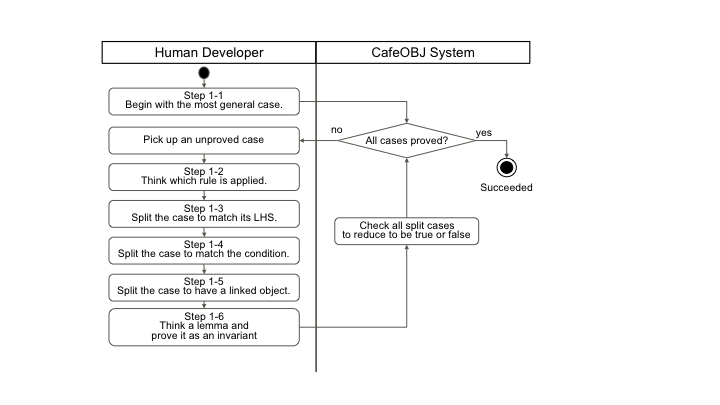
\includegraphics[height=11cm,natwidth=720,natheight=405,clip,trim=100 55 190 40]{procedure1.png}
\caption{Verification Procedure for Condition~(\ref{exp:cond1})}
\label{fig:procedure}
\end{figure}
%% ===============================================================
\section{Procedure: Proof of Condition~(\ref{exp:cond2})}
\label{sec:contcont}
%% ===============================================================
\noindent{\bf Step 2-0:} Define a predicate to be proved. \\ Using the
double negation idiom in Section~\ref{sec:searchpredicate}, predicate
{\tt contcont} for condition~(\ref{exp:cond2}) can be defined as follows.
%% =======================================================================
\begin{verbatim}
  vars S SS : State
  var CC : Bool

  pred ccont : State State
  eq ccont(S,SS)
     = inv(S) and not final(S) implies cont(SS) or final(SS) .

  pred contcont : State
  eq contcont(S)
     = not (S =(*,1)=>+ SS if CC suchThat
            not ((CC implies ccont(S,SS)) == true)
     	   { ture }) .
\end{verbatim}
%% =======================================================================

\noindent{\bf Step 2-1:} Begin with the cases each of which matches to
LHS of each rules. \\ Since condition~(\ref{exp:cond2}) checks every
possible next state of a given state $S$, we only need to prove the
cases each of which matches to each rule. For the CloudFormation
example case, we can begin with two cases for two rules as follows,
which are too general.
%% =======================================================================
\begin{verbatim}
-- Case 2.R01 of Condition (6.2) for rule R01
reduce contcont(< (res(trs,idRS,initial) sRS), sPR >) .

-- Case 2.R02 of Condition (6.2) for rule R02
reduce contcont(< (res(trs,idRRS,started) sRS), 
          (prop(tpr,idPR,notready,idRS,idRRS) sPR) >) .
\end{verbatim}

Hereafter, we only explain the steps of the procedure by omitting to show
the split case examples. \\

\noindent{\bf Step 2-2:} Split the most general case for a rule into
cases where the condition of the rule does or does not hold. \\

\noindent{\bf Step 2-3:} Split the rule applied case into cases
where predicate $final$ does or does not hold in the next state.\\

\noindent{\bf Step 2-4:} Think which rule can be applied to the next
state and repeat case splitting similarly as Step 1-3, 1-4, and 1-5
until all cases reduce to true . \\

\noindent{\bf Step 2-5:} When falling in a cyclic situation, use the
Cyclic Dependency Lemma.

%% ===============================================================
\section{Procedure: Proof of Condition~(\ref{exp:cond3})}
\label{sec:mesmes}
%% ===============================================================
Since the antecedent part of condition~(\ref{exp:cond3}) is equivalent
to~(\ref{exp:cond2}), the proof procedure of~(\ref{exp:cond3}) is
almost the same as of~(\ref{exp:cond2}). \\

\noindent{\bf Step 3-0:} Define a predicate to be proved.
\begin{verbatim}
eq mmes(S,S')
   = inv(S) and not final(S)
     implies m(S) > m(S') .
eq mesmes(S)
   = not (S =(*,1)=>+ S' if CC suchThat
        not ((CC implies mmes(S,S')) = true)) .
\end{verbatim}

\noindent{\bf Step 3-1:} Begin with the cases each of which matches to
LHS of each rule. \\

\noindent{\bf Step 3-2:} Split the most general case for a rule into
cases where the condition of the rule does or does not hold. 

%% ===============================================================
\section{Procedure: Proof of Condition~(\ref{exp:cond4})}
\label{sec:mesfinal}
%% ===============================================================
\noindent{\bf Step 4-0:} Define a predicate to be proved.
%% =======================================================================
\begin{verbatim}
eq mesfinal(S)
   = (inv(S) and (cont(S) or final(S)) and m(S) = 0)
     implies final(S) .
\end{verbatim}
%% =======================================================================
\noindent{\bf Step 4-1:} Instantiate a proved lemma. \\
The framework also provide a proved lemma such that:
%% ===============================================================
\begin{verbatim}
eq base-lemma01(SetO,ST,SetST)
   = (allObjInStates(SetO,(ST SetST)) 
      and #ObjInStates(ST,SetO) = 0)
     implies allObjInStates(SetO,SetST) .
\end{verbatim}
%% ===============================================================
Recall that {\tt allObjInStates} and {\tt \#ObjInStates} are instantiated
as {\tt allRSInStates} and {\tt \#ResourceInStates} respectively.
Since there are only two kinds of local states of resources,
\stt{allRSInStates(SetRS,(initial started))} always holds and
we can define a specific lemma as follows:
%% ===============================================================
\begin{verbatim}
eq lemma(SetRS)
   = #ResourceInStates(ST,initial) = 0 
     implies allRSInStates(SetRS,started) .
\end{verbatim}
%% ===============================================================
\noindent{\bf Step 4-2:} Use a natural number axiom.
%% ===============================================================
\begin{verbatim}
eq (N1 + N2 = 0) = (N1 = 0) and (N2 = 0) .
reduce lemma(sRS) implies mesfinal(< sRS, sPR >) .
\end{verbatim}
%% ===============================================================

%% ===============================================================
\section{Procedure: Proof of Condition~(\ref{exp:cond5}) \&~(\ref{exp:cond6})}
\label{sec:invariant}
%% ===============================================================
Since~(\ref{exp:cond5}) and~(\ref{exp:cond6}) are conditions for invariants whose proof procedure
is rather well known, here we only explain basic strategies:
\begin{itemize}
\item Prove each invariant separately but take care of dependency
  of invariants.
\item Begin with the most general case and split it by thinking
  through meaning of the specification.
\item Condition~(\ref{exp:cond6}) can be proved for each rule similarly as Step
  2-1, 2-2, and 2-3.
\item Introduce appropriate lemmas and prove them using mathematical
  induction about a set of objects.
\item Use provided lemmas, such as m2o-lemma07 explained in
  Section~\ref{sec:linklemma}.
\end{itemize}

%% ===============================================================
\section{Using Mathematical Induction for Sets of Objects}
\label{sec:induction}
%% ===============================================================

When applying the framework to verification of the example transition rule
set in Section~\ref{sec:behaviormodel}, we need to split totally 35
cases and define four invariants and four lemmas.  All lemmas are
instantiated from proved lemmas.

%% ===============================================================
\chapter{Applying the Framework to TOSCA Specifications}
\label{chap:appTOSCA}
%% ===============================================================

%% ===============================================================
\section{Structure Models of TOSCA Templates}
\label{sec:TOSCAstructure}
%% ===============================================================
We model a topology of a cloud application as a set of four kinds of
objects corresponding to the four main kinds of elements of a
topology; nodes, relationships, capabilities, and requirements. Each
object has a type, an identifier, a (local) state and may have links
to other objects. 
There is an additional object, a message pool, to represent messaging
between resources inside of different VMs because they
cannot communicate directly. The message pool is simply a bag of
messages, which abstracts implementations of messaging.

A type of nodes defines invocation rules of its operations. Each rule
specifies when an operation can be invoked and how it changes the
state of the node.  A type of relationships also defines invocation
rules of its operations. We assume that a state of a relationship is a
pair of the states of its capability and requirement in this paper for
the sake of simplicity. Thereby, an operation of a relationship type
changes the state of its capability or requirement.  As described in
Section \ref{sec:TOSCA}, type operations and their invocation rules
should be defined by type architects. When an application architect
defines a topology, the set of all type operations and the set of all
invocation rules of referred node/relationship types collectively
define behavior of the topology.

Let us use a typical example where four node types and three
relationship types in Fig.~\ref{fig:exampletopology} participate in
automation of a setup operation. In this example, we assume that
behavior of four node types is the same focusing on when a node is
created and started because they are the most essential for setup
operations.

%% ===============================================================
\section{Behavior Models of TOSCA Templates}
\label{sec:TOSCAbehavior}
%% ===============================================================
On the other hand, behavior of relationship types usually varies
according to their nature; they may be in the IaaS layer or in the
inside of VM layer, ``local'' or ``remote'', ``immediate'' or
``await''. Three relationship types of this example typically cover
the variation. A HostedOn relationship is one between resources in the
IaaS layer.  It is ``immediate'', i.e.\ it can be established as soon
as the target node is created.  Each of DependsOn and ConnectsTo
relationships is between resources inside of VMs and is ``await'',
i.e.\ it should wait for the target node to be started. A DependsOn
relationship is ``local'' in the same VM, while a ConnectsTo is
``remote'' to a different VM and should use some messages to notice
the states of its capability to its requirement.  We also assume that
types of capabilities and requirements are the same as relationships
that link them in this example for the sake of simplicity.

Behavior of these types is depicted in Fig.~\ref{fig:examplesem}.  A
solid arrow represents a state transition of each object and a dashed
arrow represents an invocation of a type operation or a message
sending.

\begin{figure}
\centering
%%\includegraphics[height=8cm]{examplesem.png}
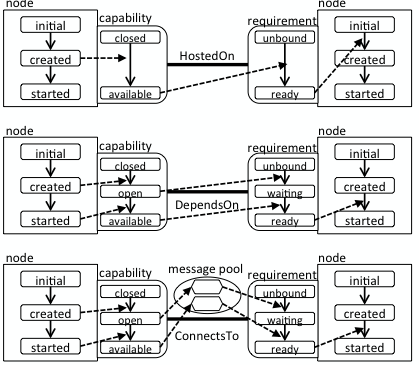
\includegraphics[height=8cm,natwidth=420,natheight=366]{./exsem.png}
\caption{Typical Behavior of Relationship Types}
\label{fig:examplesem}
\end{figure}
\begin{description}
\item[]Initial States: Every node is initially in a state named as
  $initial$, every capability of the node is $closed$, and
  every requirement is $unbound$.
\item[] Invocation Rule of Node Type Operations:
  \begin{itemize}
  \item $create$ operation can be invoked if all of the HostedOn
    requirements of the node become $ready$ and changes the state from
    $initial$ to $created$.
  \item $start$ operation can be invoked if all of the requirements
    become $ready$ and changes the state from $created$ to $started$.
  \end{itemize}
\item[] Invocation Rule of Operations of HostedOn Relationship Type:
  \begin{itemize}
  \item $capavailable$ operation can be invoked if the target node is
    already created, i.e.\ $created$ or $started$ and changes the state
    of its capability from $closed$ to $available$.
  \item $reqready$ operation can be invoked if its capability is
    $available$ and changes the state of the requirement from $unbound$
    to $ready$.
  \end{itemize}
\item[] Invocation Rule of Operations DependsOn Relationship Type:
  \begin{itemize}
  \item $capopen$ operation can be invoked if the target node is
    already created and changes the state of its capability from
    $closed$ to $open$.
  \item $capavailable$ operation can be invoked if the target node is
    $started$ and changes the state of its capability from
    $open$ to $available$.
  \item $reqwaiting$ operation can be invoked if its capability is already
    activated, i.e.\ $open$ or $available$, and the source node is
    $created$. It changes the state of its requirement from
    $unbound$ to $waiting$.
  \item $reqready$ operation can be invoked if its capability is
    $available$ and changes the state of its requirement from
    $waiting$ to $ready$.
  \end{itemize}
\item[] Invocation Rule Operations of ConnectsTo Relationship Type:
  \begin{itemize}
  \item $capopen$ operation can be invoked if the target node is
    already created. It changes the state of its capability from
    $closed$ to $open$ and also issues an open message of the
    capability to the message pool.
  \item $capavailable$ operation can be invoked if the target node is
    $started$. It changes the state of its capability from $open$ to
    $available$ and also issues an available message of the capability
    to the message pool.
  \item $reqwaiting$ operation can be invoked if it finds an open
    message of its capability and the source node is $created$. It
    changes the state of its requirement from $unbound$ to $waiting$.
  \item $reqready$ operation can be invoked if it finds an available
    message of its capability and changes the state of its requirement from
    $waiting$ to $ready$.
  \end{itemize}
\end{description}
The model described in the previous section is specified by twelve
transition rules two of which are for node operations, two are for
operations of HostedOn relationship, and eight are for four operations
of two relationship types. The followings show three of them for
$create$ and $start$ operation of nodes ({\tt R01}, {\tt R02}) and
$reqready$ operation of ConnectsTo relationship ({\tt R12}):
%% =======================================================================
\small
\begin{verbatim}
-- Create an initial node if all of its hostedOn requirements are ready.
ctrans [R01]: 
   < (node(TND,IDND,initial) SetND), SetCP, SetRQ, SetRL, MP >
=> < (node(TND,IDND,created) SetND), SetCP, SetRQ, SetRL, MP > 
   if allRQOfNDInStates(filterRQ(SetRQ,hostedOn),IDND,ready) .

-- Start a created node if all of its requirements are ready.
ctrans [R02]: 
   < (node(TND,IDND,created) SetND), SetCP, SetRQ, SetRL, MP >
=> < (node(TND,IDND,started) SetND), SetCP, SetRQ, SetRL, MP > 
   if allRQOfNDInStates(SetRQ,IDND,ready) .

-- Let a waiting ConnectsTo requirement be ready
-- if there is an available message of the corresponding capability.
trans [R12]: 
   < SetND, SetCP, 
     (req(connectsTo,IDRQ,waiting,IDND) SetRQ),
     (rel(connectsTo,IDRL,IDCP,IDRQ) SetRL), 
     (avMsg(IDCP) MP) >
=> < SetND, SetCP, 
     (req(connectsTo,IDRQ,ready,  IDND) SetRQ), 
     (rel(connectsTo,IDRL,IDCP,IDRQ) SetRL), MP > .
\end{verbatim}
\normalsize
%% =======================================================================
Here, all terms staring with capital letters are pattern-matching
variables. Since a blank character represents an associative,
commutative, and idempotent operator to construct sets with the
identity, \stt{(ND1 ND2 ND3)} represents a set of nodes and
\stt{(ND SetND)} also represents a set of nodes when
{\tt NDn} are nodes and {\tt SetND} is a set of nodes.  Predicate
\stt{allRQOfNDInStates(SetRQ,IDND,ready)} checks whether every
requirement in {\tt SetRQ} is $ready$ if the identifier of its
node is {\tt IDND}. \stt{filterRQ(SetRQ,hostedOn)} is a subset of
{\tt SetRQ} which elements are HostedOn requirements.
Note that \stt{allRQOfNDInStates(SetRQ,IDND,ready)} always holds
when node {\tt IDND} has no requirements in {\tt SetRQ}.
\stt{(avMsg(IDCP) MP)} means the message pool includes at least
one available message of capability {\tt IDCP}.
%% ===============================================================
\section{Simulation of TOSCA Templates}
\label{sec:TOSCAsimulation}
%% ===============================================================
%% ===============================================================
\section{Verification of TOSCA Templates}
\label{sec:TOSCAverification}
%% ===============================================================
A typical property of an automated system setup operation, which we
want to verify, is that the operation surely brings a cloud
application to the state where all of its component nodes are $started$.
We say ``surely'' to mean total reachability, i.e.\ any transition
sequence from any initial state always reaches some final state. Total
reachability is one of the most important properties of practical
automation of cloud applications.

The initial and final states are represented as predicates $init(S)$
and $final(S)$ that can be specified by equations in \cafeobj as
follows.
%% =======================================================================
\small
\begin{verbatim}
eq init(< SetND,SetCP,SetRQ,SetRL,MP >)
   = not (SetND = empND) and wfs(< SetND,SetCP,SetRQ,SetRL,MP >) and 
     (MP = empMsg) and allNDInStates(SetND,initial) and 
     allCPInStates(SetCP,closed) and allRQInStates(SetRQ,unbound) .
eq wfs(< SetND,SetCP,SetRQ,SetRL,MP >) 
   = allCPHaveND(SetCP,SetND) and allRQHaveND(SetRQ,SetND) and 
     allRLHaveCP(SetRL,SetCP) and allRLHaveRQ(SetRL,SetRQ) and 
     allRQHaveRL(SetRQ,SetRL) and allRLNotInSameND(SetRL,SetCP,SetRQ) .
eq final(< SetND,SetCP,SetRQ,SetRL,MP >) = allNDInStates(SetND,started) .
...
eq allRLNotInSameND(empRL,SetCP,SetRQ) = true .
eq allRLNotInSameND((RL SetRL),SetCP,SetRQ)
   = (node(getCapability(SetCP,RL)) 
      = node(getRequirement(SetRQ,RL))) = false
     and allRLNotInSameND(SetRL,SetCP,SetRQ) .
\end{verbatim}
\normalsize
%% =======================================================================
Here, we omitted definitions of several predicates;
\stt{allNDInStates(SetND,} \stt{initial)} means that every node in
{\tt SetND} is $initial$, \stt{allCPHaveND(SetCP,SetND)} means that
every capability in {\tt SetCP} has its node in {\tt SetND}, and so on.  Note
that predicate {\tt wfs} (well-formed state) specifies conditions that
should hold in not only initial states but also any reachable states.


We have proposed how to specify behavior of TOSCA topologies as state
machines and use an example state machine consisting of twelve trans
rules to verify that orchestrated operations always successfully
complete~\cite{DBLP:conf/icfem/YoshidaOF15}. For the example, we used
about 800 cases to verify the six conditions defined in
Chapter~\ref{chap:verification} and had to define 28 invariants and
many lemmas.  Here, we report how we apply the framework to the same
problem and the result.

TOSCA's four classes of object (node, relationship, capability, and
requirement) can be specified only by renaming template
{\tt OBJECTBASE}.  Links between a capability and a node, a
requirement and a node, and a relationship and a capability can be
easily specified by using template {\tt OBJLINKMANY2ONE}. Links
between a relationship and a requirement can be specified by template
{\tt OBJLINKONE2ONE}.  TOSCA distinguishes two kinds of relationships;
a local relationship is between nodes in the same VM where a remote
one is between nodes in different VMs. The capability and requirement
of a remote relationship cannot directly refer each other and instead
should communicate those local states using a messaging
mechanism. Thus, we model a global state consisting of not only the
sets of objects of four classes but also a message pool like as \stt{<
  SetND,SetCP,SetRQ,SetRL,MP >}.

19 of 28 invariants can be defined only by renaming or combining
predefined predicates. We need additional coding for the following
three reasons:
\begin{itemize}
\item Five invariants check the consistency between a message and local
states of object, e.g. if there is an available message then the
corresponding capability should be available.
\item An invariant checks the type consistency among relationships,
  capabilities, and requirement.
\item Three invariants check other problem-specific constraints, e.g.
  every node should be hosted on exactly one VM node.
\end{itemize}

The invariants defined by predefined predicates can be proved by
instantiated general lemmas of the framework. Thus, our efforts mainly
focus on proving nine other invariants, which is structured work
assisted by the verification procedure.

By using our framework, time and efforts to develop them is radically
reduced although the number of required cases is essentially the same.
Of course, it is mainly because this is our second experience of the
same problem, whereas the previous proof scores did not have any
unified policy of splitting and so were very difficult to understand
even for us. The framework makes the new proof scores become much
clear, especially those of conditions~(\ref{exp:cond2})(3)(6) which should be proved
for each of twelve transition rules.


%% ===============================================================
\chapter{Related Work and Conclusion}
\label{chap:conclusion}
%% ===============================================================
%% ===============================================================
\section{Related Work}
%% ===============================================================
%% ===============================================================
\subsection{Formal Approach for Cloud Orchestration}
%% ===============================================================
Sala{\"u}n, G., et
al.~\cite{EtcheversCBP11,SalaunBCPEG13,SalaunEPBC13} designed a system
setup protocol and demonstrated to verify a liveness property of the
protocol using their model checking method. They checked about 150
different models of system including from four to fifteen components
in which from 1.4 thousand to 1.4 million transitions are generated
and checked. They found a bug of their specification because checked
models fortunately included error cases. The model checking method can
verify correctness of checked models and so they should include all
boundary cases. In our formalization, the specification itself is
verified by interactive theorem proving in which all boundary cases
are necessary in consideration in a systematic way. It achieves
structural and deep understanding that is required to develop trusted
systems.

%% ===============================================================
\subsection{Next Version of OASIS TOSCA}
%% ===============================================================
OASIS TOSCA TC currently discusses the next version (v1.1) to define a
standard set of nodes, relationships, and operations. It is planned to
use state machines to describe behavior of the standard operations,
which is a similar approach as ours. However, the usage is limited to
clarify the descriptions of the standard and the way for type
architects to define behavior of their own types is out of the scope
of standardization. We provide a more general formalization for the
domain of cloud orchestration and also provide a framework for developing
specifications and their proofs.

%% ===============================================================
\section{Future Issues}
%% ===============================================================
While more than half of invariants and lemmas for the TOSCA
specification can be easily defined by using predefined predicates and
lemmas, extension of our framework is desired to reduce problem
specific coding and proving. The general formalization for messaging
mechanism and type system is required.

CloudFormation provides a default roll back mechanism when an
operation failure occurs but it requires manual operations when the
roll back also fails. On the other hand, the current version of TOSCA
does not manage operation failures and it focuses on declaratively
defining expected configurations of cloud applications. A possible
future extension of TOSCA may be to define alternative configurations
in failure cases, which we think we can easily extend our
formalization to handle.

In this paper, we explain our framework using examples of system setup
operations of cloud systems because cloud orchestration tools
currently focus on them. However, TOSCA is designed to be used for any
types of system operations such as scale-out and scale-in. One of the
main difficulties to specify scale-in/out operations is that they
dynamically change the structure of cloud systems, for which our
framework should be enforced from two points of view. Firstly, some
additional guidance is required to design state measuring functions,
especially for the case of scale-out where the number of resources in
the system will increase. Secondly, while the user of our framework is
left responsible for showing that \stt{noCycle(S)} is an invariant, it
may be not a trivial work as to dynamic structure. Some constraint
should be introduced in the cloud system structure to keep acyclicness
of dependency. One possible solution is to assume a partial order of
types of objects and to allow transition rules to produce dependency only
in the descending order.

%% ===============================================================
\section{Conclusion}
%% ===============================================================
A general formalization of declarative cloud orchestration is proposed
and a framework is provided for interactive developing proof
scores. The framework provides a general model and a procedure for
verifying leads-to properties of declarative cloud orchestration.  The
procedure systematically assists the verification process and makes
its generic part be routine work whose efforts are reduced by the
provided logic templates and predicate libraries. As a result, a
verification engineer can concentrate on the work specific to the
individual problem.

A related work applied their model checking method to a typical
problem in the domain of cloud orchestration, in which many of
finite-state systems were checked. Our framework is more general to be
applied to different kinds of models in the domain and to be used for
interactive theorem proving which can verify systems of arbitrary many
number of states in a significantly systematic way.

All \cafeobj codes of the framework and example proof scores
can be downloaded at \url{https://github.com/yuki-yoshida/JAIST}.

\appendix

\bibliographystyle{plain}
\bibliography{DThesis}

\begin{publication}
\addcontentsline{toc}{chapter}{Publications}

\item
Hiroyuki YOSHIDA, Kazuhiro OGATA, and Kokichi FUTATSUGI,
Formalization and Verification of Declarative Cloud Orchestration,
\emph{Formal Methods and Software Engineering - 17th International Conference
               on Formal Engineering Methods, {ICFEM} 2015, Proceedings}, 
Lecture Notes in Computer Science 9407,
pp 33-49, 
Springer,
Paris, France,
November 3-5, 2015

\end{publication}
\end{document}
